%\documentclass[final,5p,times,twocolumn]{elsarticle}
\documentclass[smallextended]{svjour3}
%\biboptions{numbers,sort&compress}
%\documentclass[sigconf,review, anonymous]{acmart}
%\hyphenation{on-tol-o-gy ad-di-tion-al in-fra-struc-ture an-a-lyze a-nal-y-sis}
%


\usepackage{inconsolata}
\usepackage{listings}

\lstset{language=Java,
basicstyle=\ttfamily\scriptsize,
%basicstyle=\ttfamily,
keywordstyle=\color{javapurple}\bfseries,
stringstyle=\color{pblue},
commentstyle=\color{javagreen},
morecomment=[s][\color{javadocblue}]{/**}{*/},
morecomment=[s][\color{gray}]{@}{\ },
numbers=left,
numberstyle=\tiny\color{black},
stepnumber=2,
numbersep=8pt,
tabsize=4,
showspaces=false,
showstringspaces=false,
breaklines=true,}

%%%%%%%%%%%%%%%%%%%%%%%%%%%%%%%%%%




\usepackage{adjustbox} % ajustar tabela ao tamanho da pagina

\usepackage{tikz}
\usetikzlibrary{matrix,fit,shapes,calc,positioning,shadows,arrows,shapes,backgrounds,decorations.markings,fadings}
\usepackage{graphicx}
\usepackage{multirow}
\usepackage[caption=false, font=footnotesize]{subfig}
\usepackage{wrapfig}
\usepackage{enumitem}
\usepackage{url}

%%%%%%%%%%%%%%%%%%%%%%%%%%%%%%%%%%%%%%%%%%%%%%%%%%%%%%%%%%%%
%% Comment the \draftmodetrue line before submission
%%%%%%%%%%%%%%%%%%%%%%%%%%%%%%%%%%%%%%%%%%%%%%%%%%%%%%%%%%%%
\newif\ifdraftmode
\draftmodetrue

%% avoid footnotes across pages
\interfootnotelinepenalty=10000
%\raggedbottom

%%%%%%%%%%%%%%%%%%%%%%%%%%%%%%%%%%%%%%%%%%%%%%%%%%%%%%%%%%%%
%% Uncomment \showsplattexttrue to show text from our splat paper
%%%%%%%%%%%%%%%%%%%%%%%%%%%%%%%%%%%%%%%%%%%%%%%%%%%%%%%%%%%%
\newif\ifshowsplattext
%\showsplattexttrue

\pagenumbering{arabic}

%% paragraphs within margins
\usepackage[english]{babel}
\setlength{\emergencystretch}{2pt}
\usepackage{booktabs}
\usepackage{multirow}
\usepackage{tikz}
\usepackage{xspace}
\usetikzlibrary{matrix,fit,shapes,calc,positioning,shadows,arrows,shapes,backgrounds,decorations.markings,fadings}
\usepackage{listings}
\usepackage[caption=false, font=footnotesize]{subfig}
%%%%%%%%%%%%% code listing
\renewcommand{\ttdefault}{pcr}
\lstset{
  basicstyle=\scriptsize\ttfamily,
  keywordstyle=\scriptsize\ttfamily\bfseries,
  language=Java,             % choose the language of the code
  frame=single,              % adds a frame around the code
  aboveskip=0pt,
  belowskip=0pt,
  breaklines=true,           % sets automatic line breaking
  breakatwhitespace=false,   % sets if automatic breaks should only happen at
  showspaces=false,
  %numbersep=5pt,              % Abstand der Nummern zum Text
  %tabsize=2,                  % Groesse von Tabs
  %extendedchars=true,         %
  %breaklines=true,            % Zeilen werden Umgebrochen
  keywords=[2]{class, incorporateUserFeedback, testPushPop, testPopPush},
}
\usepackage{balance}
\usepackage{wrapfig}
\usepackage{enumitem}
\usepackage{url}

%% helpers
\newcommand{\js}{JS}
\newcommand{\javascript}{JavaScript}
\newcommand{\es}{ES}
\newcommand{\ecmascript}{\es{}}
\newcommand{\tname}{TNAME}
\newcommand{\Comment}[1]{}
\newcommand{\numsubjects}{5}
\newcommand{\etal}{and colleagues'}
\newcommand{\ie}{i.e.}
\newcommand{\eg}{e.g.}
\newcommand{\cmark}{\ding{51}}%
\newcommand{\xmark}{{\color{red}\ding{55}}}%
\newcommand{\pGoodGood}{$\mathit{P}${\small\cmark\!\cmark}}%
\newcommand{\pGoodBad}{$\mathit{P}${\small\cmark\!\xmark}}%
\newcommand{\pBadDontCare}{$\mathit{P_?}$}%
\newcommand{\sfl}{SFL\xspace}
\newcommand{\ddg}{DDG\xspace}
\newcommand{\totfiles}{$\sim$38K}

%% annotations
\newif\ifdraftmode
%% Comment or uncomment the \draftmodetrue line.
\draftmodetrue
\ifdraftmode
 \newcommand{\Fix}[1]{\textbf{[[}{\color{red} #1}\textbf{]]}}
 \newcommand{\Mar}[1]{\textbf{[[Marcelo: }{\color{magenta} #1}\textbf{]]}}
 \newcommand{\Igor}[1]{\textbf{[[Igor: }{\color{blue} #1}\textbf{]]}}
 \newcommand{\note}[1]{\todo[inline,color=red!30,caption={}]{#1}}
\else
 \newcommand{\Fix}[1]{\relax}
 \newcommand{\Mar}[1]{\relax}
 \newcommand{\Igor}[1]{\relax}
 \newcommand{\note}[1]{\relax}
\fi

% For submitted version only.
\pagenumbering{arabic}

% Uncomment this if you need more space
%% \makeatletter
%% \def\@copyrightspace{\enlargethispage{-10pt}\relax}
%% \makeatother

\newcommand{\codesize}{\small}
\newcommand{\CodeIn}[1]{\mcodeid{#1}}
\newcommand{\CodeInM}[1]{\mcodeid{#1}}
% \|name| or \mathid{name} denotes identifiers and slots in formulas
\def\|#1|{\mathid{#1}}
\newcommand{\mathid}[1]{\ensuremath{\mathit{#1}}}
% \<name> or \codeid{name} denotes computer code identifiers
\def\<#1>{\codeid{#1}}
\newcommand{\codeid}[1]{\ifmmode{\mbox{\codesize\ttfamily{#1}}}\else{\codesize\ttfamily #1}\fi}
\def\<#1>{\mcodeid{#1}}
\newcommand{\mcodeid}[1]{\mbox{\codesize\ttfamily{#1}}}

%% thumbs up down
\newcommand*{\RightThumbsUpAux}[1]{%
  \begingroup
    \sbox0{Ag}%
    \raisebox{-\dp0}{%
      \includegraphics[{%
        height=\dimexpr\dp0+\ht0\relax,
        #1%
      }]{thumbsup.pdf}%
    }%
  \endgroup
}
\newcommand*{\RightThumbsUp}{%
  \RightThumbsUpAux{}%
}
\newcommand*{\RightThumbsDown}{%
  \RightThumbsUpAux{origin=c,angle=180}%
}
\newcommand*{\LeftThumbsUp}{%
  \scalebox{-1}[1]{\RightThumbsUp}%
}
\newcommand*{\LeftThumbsDown}{%
  \scalebox{-1}[1]{\RightThumbsDown}%
}

\newcommand{\checkm}{Y}
\newcommand{\crossmark}{N}
%\begin{wraptable}[20]{t}[0pt]{0.5\textwidth}

\newcommand{\totalTestFiles}{38,369}
\newcommand{\totalTestFilesCompileInAll}{35,939}
\newcommand{\totalTestFilesPassInAll}{24,493}
\newcommand{\nofuzzAll}{209}
\newcommand{\nofuzzBugs}{\Fix{XX}}
\newcommand{\nofuzzDuplicates}{63}
\newcommand{\nofuzzFalsePositives}{24}
\newcommand{\nofuzzHITotal}{177}
\newcommand{\nofuzzLOTotal}{32}
\newcommand{\nofuzzTotalFiles}{977} % conflicting files
\newcommand{\nofuzzFilesHI}{940} % conflicting files HI
\newcommand{\nofuzzFilesLO}{37} % conflicting files LO

\newcommand{\nofuzzBucketsBugsHI}{\Fix{124}} % buckets reported (including dups)
\newcommand{\nofuzzBucketsBugsLO}{\Fix{11}} % buckets reported
\newcommand{\nofuzzDupsHI}{\Fix{X}}
\newcommand{\nofuzzDupsLO}{\Fix{Y}}

% continue updating bugs table
\newcommand{\tableBugsNum}{\Fix{26}}

%% anonymize

\newcommand{\anonym}[1]{{\tiny\colorbox{black}{#1}}}

%% names
\newcommand{\radamsa}{radamsa}
\newcommand{\quickfuzz}{quickfuzz}

\newcommand{\jsc}{JavaScriptCore}
\newcommand{\veight}{V8}
\newcommand{\chakra}{Chakra}
\newcommand{\smonkey}{SpiderMonkey}
\newcommand{\jerry}{JerryScript}

\newcommand{\lo}{lo}
\newcommand{\hi}{hi}


\journalname{Software Quality Journal}

\begin{document}

%\title{Leveraging Diversity to Find Bugs in JavaScript Engines}
\title{Exposing Bugs in JavaScript Engines through Test Transplantation and Differential Testing}
\titlerunning{Exposing Bugs in JavaScript Engines}        % if too long for running head

\author{Igor Lima \and Jefferson Silva \and Breno Miranda\footnotemark
  \and Gustavo Pinto \and Marcelo d'Amorim}
%\authorrunning{Short form of author list} % if too long for running head

\institute{
* Corresponding author: Breno Miranda \and
\email{bafm@cin.ufpe.br}\\ \\
Igor Lima \and \email{isol2@cin.ufpe.br} \\
Jefferson Silva \and \email{jefferson.alves.silva@icen.ufpa.br}\\
Breno Miranda \and \email{bafm@cin.ufpe.br} \\
Gustavo Pinto \and \email{gpinto@ufpa.br} \\
Marcelo d'Amorim \and \email{damorim@cin.ufpe.br} \\
\at Universidade Federal de Pernambuco, Recife, PE, Brazil}

\date{Received: date / Accepted: date}
% The correct dates will be entered by the editor

%\institute{Corresponding author.}


%\renewcommand{\shortauthors}{Lima et al.}

\maketitle

\begin{abstract}
  JavaScript is a popular programming language today. Several engine
implementations compete for market dominance. Although specification
and conformance test suite exist to guide engine development, bugs
occur and have important consequences given the language
popularity. One reason for the difficulty in implementing correct
engines stems from the fact that the specification is incomplete and
evolves frequently.

This paper reports on a study we ran to evaluate the importance of
diversity in finding bugs on JavaScript engines. For that, we explored two
simple diversity-aware methods---test transplantation and cross-engine
differential testing. Test transplantation evaluates the effects of
running test suites of a given engine in another engine. Cross-engine
differential testing evaluates the effects of fuzzing existing inputs
and then comparing the output produced by different engines with a
differential oracle.

We considered engines from four major players in our
experiments--Apple, Google, Microsoft, and Mozilla. Our results
indicate that both techniques revealed several bugs, most of which
confirmed by developers. Test transplantation
revealed \noBugsTransplantation{} bugs
(\noBugsTransplantationConfirmed{} confirmed) and differential testing
revealed \noBugsDifferentialTesting{} bugs
(\noBugsDifferentialTestingConfirmed{}). Furthermore, results indicate
that most of these bugs affected only two engines--Apple's
\jsc{} (\percJSC{}) and Microsoft's \chakra{} (\percChakra{}); we found
only one bug in Google \veight{} and none in Mozilla's
\smonkey{}. Although our experience indicates that more research needs
be done to automate parts of the inspection process, our results show
that exploring diversity is a valuable help to find bugs in JavaScript
engines.

  %\keywords{Diversity \and Test Transplantation \and Differential Testing \and JavaScript}
  \keywords{Test Transplantation \and Differential Testing \and JavaScript}
\end{abstract}

\section{Introduction}

JavaScript (\js{}) is one of the most popular programming languages
today~\cite{stackify,redmonk-javascript}, with penetration in various
software development segments including, web, mobile, and, more
recently, the Internet of Things~(IoT)~\cite{simply-technologies}. The
interest of the community for the language encourages constant
improvements in its specification~\cite{ecmas262-spec}. It is natural
to expect that such improvements lead to sensible changes in engine
implementations~\cite{kangax}. Even small changes can have high
practical impact. For example, in October 2014 a new attribute added
to Array objects resulted in the MS Outlook Calendar web app to fail
under Chrome~\cite{array-bug-chromium-issue4247,array-bug-discussion}.

Finding bugs in \js\ engines is an important problem given the range
of applications that could be affected with those bugs. It is also
challenging.  Specifications are intentionally incomplete as to enable
development flexibility. In addition, they evolve frequently to
accommodate the pressing demands from
developers~\cite{ecmas262-spec-repo}. An official conformance test
suite exists for \js~\cite{tc39-github}, but, naturally, many test
scenarios are not covered in the suite. In addition, we noticed that a
significant fraction (5 to 15\%) of the tests in that suite fail
regularly in the most popular engines, reflecting the struggle of developers in keeping
up with the pace of spec evolution (see Table~\ref{tab:test262}).

%% WHAT WE DID
This work, which is empirical in nature, reports on a study to evaluate
the ability of two testing techniques to expose bugs in JavaScript engines.

%\vspace{-1ex}
%noitemsep,
\begin{itemize}[topsep=0pt,parsep=0pt,partopsep=2pt,labelwidth=0cm,align=left,itemindent=-0.25cm]
\item \emph{Test transplantation}.
  This technique evaluates the effect of running test files
  written for a given engine in other engines. The intuition is that
  developers design test cases with different objectives in mind. As
  such, replaying these tests in different engines could reveal
  unanticipated problems.

\item \emph{Cross-engine differential testing}.  This technique fuzzes
  existing test inputs~\cite{fuzz-testing-history} and then compares
  the output produced by different engines using a differential
  oracle. The intuition is that interesting inputs can be created from
  existing inputs and multiple engines can be used to address the lack
  of oracles for the newly created inputs.
\end{itemize}

The study measures the ability of these techniques in finding bugs and
the impact of false positives on their practicality. \Mar{seria bom
  adicionar uma frase com rationale para escolha destas tecnicas.}

%One of
%various causes of output discrepancy is a bug.

%% It automates test generation in scenarios where multiple
%% implementations of a system exist. DT leverages diversity across
%% system's implementations to detect anomalous behavior.
%\emph{Related Ideas.}~The idea of test set diversity dates back to the
%eighties~\cite{white-cohen-tse1980,ostrand-balcer-1988}. In contrast
%to prior work on this topic, this paper explores diversity of
%implementations and diversity of sources of test cases as opposed to
%diversity of the test cases themselves. Section~\ref{sec:related:diversity-testing}
%elaborates related work on this topic.
%
\emph{Related Ideas.}~Differential Testing~\cite{Brumley-etal-ss07}
(DT) has been applied in a variety of contexts to find
bugs~\cite{Yang-etal-pldi11,Chen-etal-fse2015,Argyros-etla-ccs16,Chen-etal-pldi16,petsios-etal-sp2017,SivakornAPKJ17,Zhang:2017:ATD:3097368.3097448}.
It has shown to be specially practical in scenarios where the
observation of difference gives a strong signal of a real problem. For
example, Mozilla runs JS files against different configurations of a
given build of their \smonkey\ engine (\eg{}, trying to enable or not
eager JIT compilation\footnote{These files are created with the
  grammar-based fuzzer jsfunfuzz~\cite{jsfunfuzz}. Look for option
  ``compare\_jit'' from funfuzz.}). A positive aspect of the approach
is that it can be fully automated---as only one engine is used, the
outcomes of the test in both configurations are expected to be
identical. The Mozilla team uses this approach since 2002; they have
been able to find over 270 bugs since
then~\cite{jsfunfuzz-at-mozilla}, including security
bugs. Cross-engine differential testing, in contrast, has not been
widely popularized because the reported differences are more unlikely
to be false alarms. In this context, a number of legitimate reasons
exist, other than a bug, for a test execution to manifest discrepancy
(see Tables~\ref{fig:piecharts-transplantation} and
~\ref{tab:false-positives}). As consequence, humans need to inspect
the reports.

%Variations of these ideas have been explored before in different contexts.

%It is important to note that the goal of the paper is to assess the
%ability of the techniques aforementioned in finding bugs on \javascript\ engines.

%% This paper evaluates the benefits of
%% test case diversity and engine diversity in finding bugs on
%% \javascript\ engines.

%% Recently, Patra and
%% Pradel~\cite{patra2016learning} proposed a language-agnostic fuzzer to
%% find cross-browser HTML+JS discrepancies. The main difference of our
%% work to theirs is in goal; our goal is to evaluate ability and cost of
%% simple diversity-aware approaches to find bugs in \js\ engines.

%% Their main contribution was
%% analytical whereas our main contribution is empirical--

\begin{figure}[t]
%  \vspace{-2ex}
  \centering
  \subfloat[\label{fig:stacked-engine}Bug reports per engine.]{
    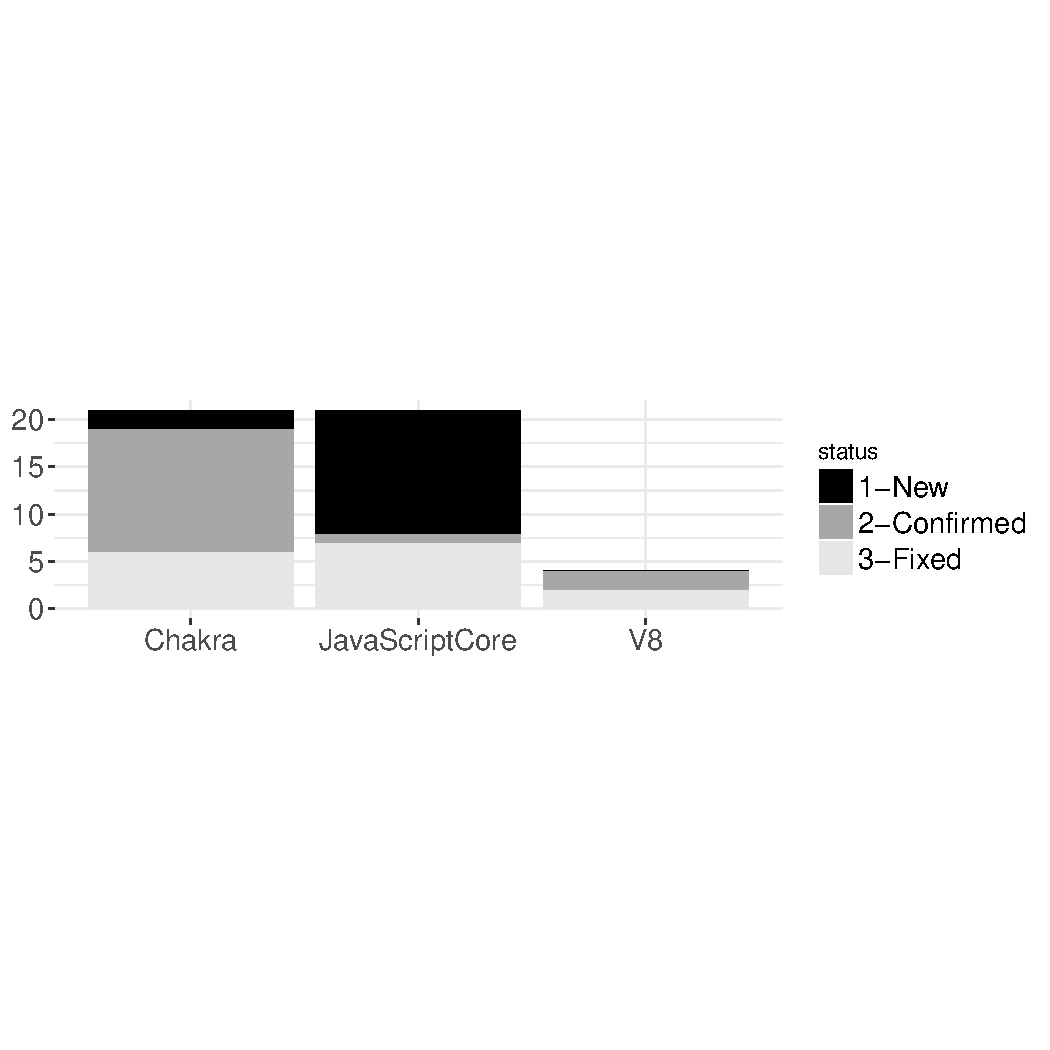
\includegraphics[trim=0 150 0 180,clip,width=\textwidth,scale=0.4]{R/stackedbar/stacked-engine}
    \vspace{-5ex}
  }\\
  \subfloat[\label{fig:stacked-technique}Bugs reports per technique.]{
    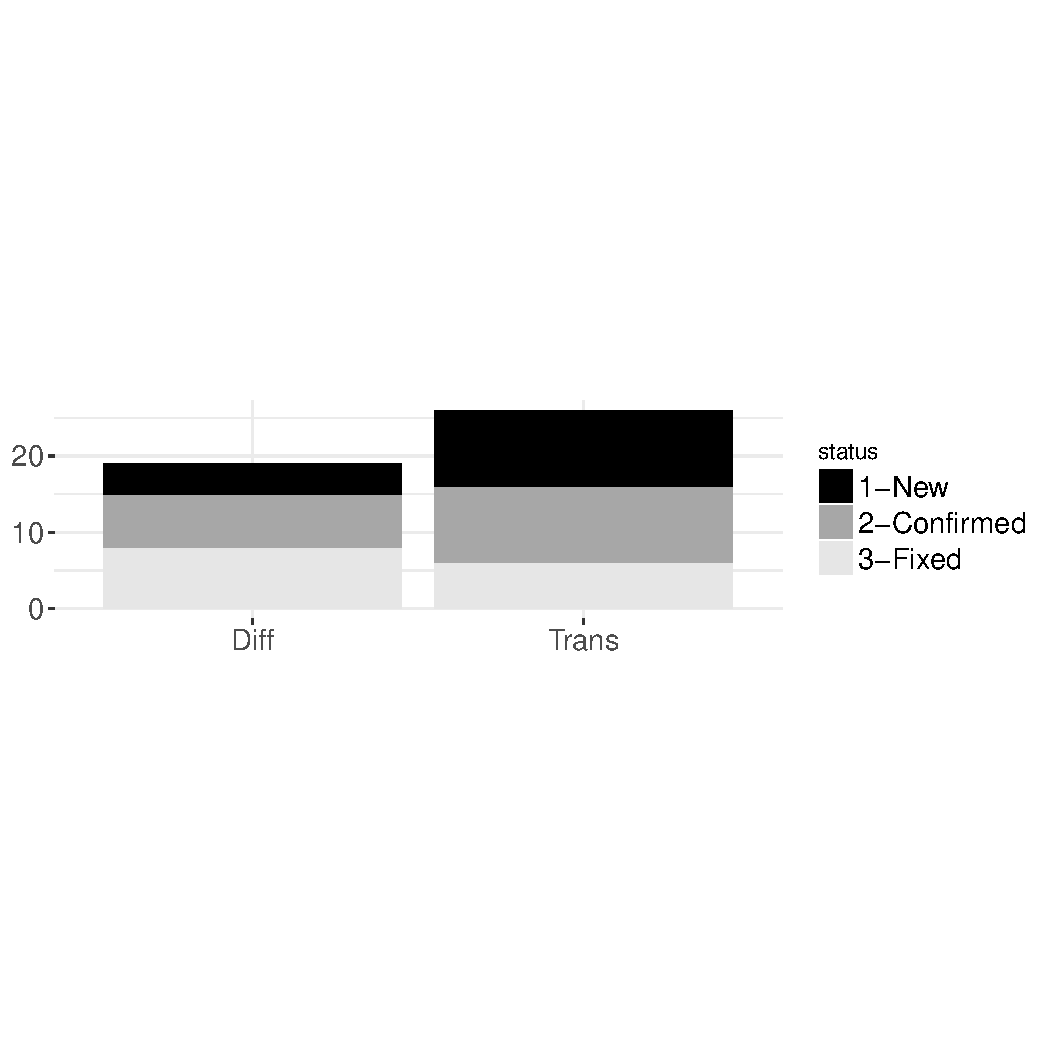
\includegraphics[trim=0 150 0 180,clip,width=0.7\textwidth,scale=0.4]{R/stackedbar/stacked-technique}
    \vspace{-5ex}
  }
  \caption{\label{fig:summary}Summary of bug reports.}
  \vspace{-3ex}
\end{figure}

\sloppy \emph{Results.}~We considered the following engines--\chakra{}
(Microsoft), JavaScriptCore (Apple), \veight{} (Google),
\smonkey{} (Mozilla), and \hermes (Facebook). Figure~\ref{fig:summary} shows the breakdown of bug reports per engine (\ref{fig:stacked-engine}) and per technique
(\ref{fig:stacked-technique}).
Each stacked bar breaks down the bugs
per status (\eg{}, ``1-New''). The prefix number indicates the
ordering that status labels are assigned. Several of these
reports have the label ``3-Fixed'', indicating that bug fixes have
been incorporated into the code already. Note that most of these bugs
affected two engines--\chakra{} and JavaScriptCore (\jsc).  We
reported \noBugsBugsReportedGoogle{} bugs in \veight{}
(\noBugsBugsConfirmedGoogle{} confirmed),
\noBugsBugsReportedHermes in \hermes,
and \noBugsBugsReportedSMonkey in \smonkey{}.
Furthermore, our results show that both techniques revealed several
bugs, most of which confirmed by developers. Test transplantation
revealed \noBugsTransplantation bugs (of which,
\noBugsTransplantationConfirmed were confirmed and
\noBugsTransplantationFixed were fixed) whereas differential testing
revealed \noBugsDifferentialTesting bugs (of which,
\noBugsDifferentialTestingConfirmed were confirmed and
\noBugsDifferentialTestingFixed were fixed).  Overall, results
indicate that both techniques were successful at finding bugs. The
number of bug reports were similar, if we consider only those
confirmed or fixed. Most bugs we found are of moderate severity.

%% Considering cost per bug found, we found that test
%% transplantation, compared to differential testing, demanded less
%% effort from the developers who inspected the alarms.

%% All in all, these simple techniques
%% seem promising to improve reliability of engines that continuously
%% evolve with their specifications.

\emph{Key Findings.}~We found that--1)~Differential testing and Test
Transplantation are practical and effective techniques to find bugs on real,
complex, and widely used software systems, 2)~Even for problems with
fairly clear specifications, as in \javascript{}, there is likely (a
lot of) variation between different implementations, which brings intrinsic
challenges to developers that work on them.
Section~\ref{sec:lessons} expands and elaborates key
findings and lessons learned.

%% LIST OF CONTRIBUTIONS
\emph{Contributions.}~The most important contribution of this work is empirical:
we provide a comprehensive study analyzing the effectiveness of
test transplantation and differential testing
in revealing functional bugs in popular \javascript\ engines.
Additional contributions are:
1)~A number of bugs found and fixed.
We reported a total of \totalBugsReported bugs.
Of these, \totalBugsConfirmed bugs were confirmed and \totalBugsFixed bugs were fixed.
2)~An infrastructure for performing test transplantation and differential testing.
Both the scripts to run the experiments and the data processed are publicly available at \dataRepo.

\vspace{1ex} To summarize, this paper provides initial, yet strong evidence
that exploring test transplantation and differential testing
should be encouraged to find functional bugs
in JavaScript engines.

\section{JavaScript}
\label{sec:es6-design}
\label{sec:imp-dep-behavior}

JavaScript engines are virtual machines that parse source code,
compile it in bytecodes, and run these bytecodes. These engines
implement some version of the ECMAScript (\es{}), which emerged with
the goal to standardize variants of the language, such as Netscape's
JavaScript and Microsoft's JScript\footnote{The name JavaScript still
  prevails today, certainly for historical reasons.}. The \es{}
specification is regulated by Ecma International~\cite{es6-website}
under the TC39~\cite{tc39-github} technical committee.  Every year, a
new version of the \es{} specification is produced with new features
and minor fixes. The canonical spec today is
ES6~\cite{ecmas262-spec-repo,ecmas262-spec}.

%% In the following, we briefly describe different sources of
%% discrepancies that can emerge across different engine implementations
%% as results of the active changes in the \es{} specification.
%% .........
%% A compatibility table relating features and supporting engines is
%% publicly available~\cite{kangax}.

The specification of JavaScript is incomplete for different
reasons. Certain parts of the specification are undefined; it is
the responsibility of engineers to decide how to implement these
functionalities. The JavaScript spec uses the label
``implementation-dependent'' to indicate these cases, where behavior
may differ from engine to engine. One reason this flexibility in the
spec exists to enable compiler optimizations. For example, the
\js\ \mcodeid{for-in} loop construct does not clearly specify the
iteration order of
elements~\cite{so-forin-undefined,javascript-in-chrome} and different
engines capitalize on that for loop
optimizations~\cite{for-in-undefined}.  As another example, the
specification states that if the \mcodeid{Number.toPrecision()}
function is called with multiple arguments then the floating-point
approximation is
implementation-dependent~\cite{es6-toPrecision}. Various other cases
like these exist in the specification. Given the speed the
specification changes and the complexity of the language some features
are not fully implemented as can be observed by the Kangax
compatibility table~\cite{kangax}.  It is also worth noting that, as
in other languages, some elements in JS have non-deterministic
behavior (\eg{}, \mcodeid{Math.random} and \mcodeid{Date}). A test
that makes decisions based on these elements could, in principle,
produce different outcomes on different runs. Carefully-written test
cases should not manifest this kind of flaky behavior.  As previously
mentioned, all those aspects make testing \js\ engines challenging.


%\subsection{Randomness}


%\subsection{\Fix{Other}}

%% 1) The stack depth in JS is often close to the real (native) C stack
%% depth, nevertheless observable by JS through recursion. This causes
%% differential behavior even on the same engine when JITs are enabled or
%% disabled, as the stack frame sizes vary. LangFuzz in particular
%% produces a lot of recursions and hits these problems even more often
%% than jsfunfuzz.\Mar{ask C. Holler. it is unclear to me how the output
%%   could be different.}

%% \section{Objects of Study}
%% This section discusses the objects we used in our study.

\section{Engines Studied}
\label{sec:methodology}
\label{sec:methodology:engines}~We selected
JS engines according to the following criteria: 1) Released latest
version after Jan 1, 2018, 2) Contains more than 1K stars on GitHub,
and 3) Uses a public issue tracker. We looked for highly-maintained
(as per the first criterion) and popular (as per the second criterion)
engines. As we wanted to report bugs, we also looked for project with
public issue trackers. Table~\ref{tab:engines} lists the engines we
analyzed. It is worth noting that we used Google Chrome Lab's JSVU
tool~\cite{jsvu} to automatically install and configure versions of
different JS engines in our host environment. This is important as we
aim to use the most recent stable versions of each engine as to avoid
reporting old and already-fixed bugs to developers.

%% Table~\ref{tab:engines} shows the engines we selected in this
%% study. We made an exception to the second criterion with
%% XS~\cite{xs2018repo}. As the project is young, created in Oct 2017, we
%% thought there was insufficient time to obtain 1K stars for XS. We
%% still considered this project as it seems to be attracting interest
%% from the community\Fix{is this true?}

\begin{table}[t]
  \small
  \centering
  \caption{\label{tab:engines}Engines selected.}
  \begin{tabular}{cccrrr}
    \toprule
    Team & Name & URL & \# Stars  & DOB \\
    \midrule
    Apple & \jsc (WebKit) & \cite{jsc2018repo} & 3300+ & Jun 2001 \\
    Google & \veight{} & \cite{v82018repo} & 9800+ & Jun 2008 \\
    Microsoft & \chakra{} & \cite{chakra2018repo} & 7200+ & Nov 2009 \\
    Mozilla & \smonkey{} & \cite{spidermonkey2018repo} & 1100+ & Mar 1996 \\
    Facebook & \hermes & \cite{hermes2020repo} & 5400+ & Jul 2019 \\
   \bottomrule
  \end{tabular}
\end{table}

% hermes very first commit: https://github.com/facebook/hermes/commit/f22a18f67da3f03db59c1ec715d6ec3776b03fbf

\section{Mined JS Files}
\label{sec:seeds}
A good test set is critical for finding bugs with the techniques used
in this paper. For that reason, we looked for \js\ files from various
sources: 1) test files from the Test262~\cite{tc39-github} conformance
suite of the ECMA262 specification~\cite{ecmas262-spec}, 2) test files
from the test suite of the selected engines (see
Section~\ref{sec:methodology:engines}); these files are accessible
from the engine's official repositories, 3) test files from the suites
of public engines (\ie{}, Duktape, JerryScript, JSI, and Tiny-js),
4) test files mined from issue trackers of
these engines, and 5) test files from other GitHub projects.

%% accessible from GitHub using the GitHub REST
%% API~\cite{github-rest-api}.

Table~\ref{tab:test-suites} shows the breakdown of tests per
engine. Column ``full'' shows the number of test cases associated with
each engine. Column ``pass-in-par.''  shows the number of test cases
that pass in their parent engine. We discarded tests that fail in
their parent engine as we could not reliably indicate the reason for
the failure, so we assumed the test could be broken. We removed \testsThatFail{}
test cases that fail for that reason--\testsThatFailJSC{} tests from \jsc and
\testsThatFailSM{} tests from \smonkey. Column ``type-in-all''
shows the number of test cases whose executions do not throw
dynamic type errors in any of the engines because of an undefined variable or property.
These cases were captured by looking for the presence of \CodeIn{ReferenceError} and
\CodeIn{TypeError} in the output. A \CodeIn{ReferenceError}
(respectively, \CodeIn{TypeError}) is raised when test execution
attempts to access an undefined variable (respectively, property of an
object). We discarded those tests to avoid noise in the experiments as
they clearly indicate some missing feature as opposed to bugs. For
example, some tests use non-portable names (\eg{}, \jsc's
\CodeIn{drainMicrotasks()} and \smonkey{}'s \CodeIn{Error.lineNumber})
or use functions that, albeit part of the spec, not all engines
currently support. \Fix{Similarly, the \chakra project does not use the default
well-known assertions available in JS, which the other JS engines use.
Instead, it uses its own testing framework, WScript. In this case, we could
not easily reproduce the \chakra unit tests in the other engines since it would
raise a \texttt{ReferenceError}. Also, updating the other engines to use WScript would
require a non-trivial manual process. This is why \chakra is not showed
in Table~\ref{tab:test-suites}.}

For the evaluation of test transplantation, we used
the \totalTestFilesForTestTransplantation{} tests included in the
dashed rectangle under column ``type-in-all'', \ie{}, all tests under
that column but the Test262 tests. We did not consider tests from the
conformance suite as they are more likely to indicate missing features
as opposed to bugs. In addition, engine developers have access to
these test and are encouraged to run them. Finally, column
``no-fail-in-all'' shows the tests for which all engines pass. Note
that the set of tests in this column is a subset of the
``type-in-all'' test set. This test set is used in the evaluation of
differential testing as fuzzing seeds. The guarantee that they pass in
all engines assures that, if discrepancies occur, they are related to
the changes in the input as opposed to the original cause of failure.

\newcommand\marktopleft[1]{%
    \tikz[overlay,remember picture]
        \node (marker-#1-a) at (0,2ex) {};%
}
\newcommand\markbottomright[1]{%
    \tikz[overlay,remember picture]
        \node (marker-#1-b) at (0,0) {};%
    \tikz[overlay,remember picture,thick,dashed,inner sep=2pt]
        \node[draw,rectangle,fit=(marker-#1-a.center) (marker-#1-b.center)] {};%
}

\begin{table}[t]
  \small
  \centering
  \caption{\label{tab:test-suites}Number of test files. Dashed
    rectangle under column ``type-in-all'' (resp., ``no-fail-in-all'')
    shows the tests used for test transplantation (resp., cross-engine
    differential testing).\Gustavo{Terminar essa tabela}}  \setlength{\tabcolsep}{2pt}
  \begin{tabular}{ccrrrr}
    \toprule
    \multirow{2}{*}{Name}      &  \multirow{2}{*}{Source} &
    \multicolumn{4}{c}{\# JS files} \\
    \cline{3-6}
                               &         & total & pass-in-par. & type-in-all &  no-fail-in-all \\
    \midrule
    Test262 & \cite{ecma262-conformance-suite} & \testOriginal{} & \testPassInPar{} &  \testCompileAll{} & \marktopleft{c2}\testNoFailAll{} \\
    \midrule
    \jsc & \cite{jsc2018repo} & \jscOriginal{} & \jscPassInPar{} &\marktopleft{c1}\jscCompileAll{} & \jscNoFailAll{}\\
    \smonkey\ & \cite{mozilla} & \smOriginal{} & \smPassInPar{} & \smCompileAll{} & \smNoFailAll{}\\
    \veight{} & \cite{v82018repo} & \veightOriginal{} & \veightPassInPar{} & \veightCompileAll{} & \veightNoFailAll{}\\
    %\chakra & \cite{chakra2018repo}\\
    \hermes & \cite{hermes2020repo} & \hermesOriginal{} & \hermesPassInPar{} & \hermesCompileAll{} & \hermesNoFailAll{} \\
    \midrule
    Duktape & \cite{duktape} & \duktapeOriginal{} & \duktapePassInPar{} & \duktapeCompileAll{} & \duktapeNoFailAll{}\\
    \jerry{} & \cite{jerryscript2018repo} & \jerryOriginal{} & \jerryPassInPar{} & \jerryCompileAll{} & \jerryNoFailAll{}\\
    JSI & \cite{jsi} & \jsiOriginal{} & \jsiPassInPar{} & \jsiCompileAll{} & \jsiNoFailAll{}\\
    Tiny-js & \cite{tinyjs} & \tinyOriginal{} & \tinyPassInPar{} & \tinyCompileAll{}\markbottomright{c1} & \tinyNoFailAll{}\markbottomright{c2}\\
    \midrule
    GitHub Projects & - & 494,394 & - & - & - \\
    \midrule
     &  & \totalTestFiles{} & \totalTestFilesPassInPar{} & \totalTestFilesCompileInAll{} & \totalTestFilesPassInAll{}\\
   \bottomrule
  \end{tabular}
\end{table}


%% The main source of test
%% cases is the official Test262~\cite{tc39-github} conformance test
%% suite for the ECMA262 specification~\cite{ecmas262-spec}.\Comment{
%%   This test suite contains 87\% of all the tests we used.} We also
%% considered test suites of three of the four engines mentioned in
%% Section~\ref{sec:methodology:engines} and four other engines. Overall,
%% we selected a total of \totfiles{} JS
%% files.

\lbrack{}Cleansing\rbrack{}~We noticed that some of the tests we found
depend on external libraries, which not all selected engines
support. We decided to discard those. For example, many tests we found
required a Node.js runtime~\cite{node} for execution. Also, we did not
consider tests from the \chakra{} repository because they depend on
non-portable objects.
Finally, note that the number of tests in
\veight\ is low; that happens because \veight{} uses many tests from
Mozilla and \jsc; we discarded those to avoid repetition and to give
credit where it is due. \lbrack{}Test Harness\rbrack{}~It is also
worth mentioning that some engines use a custom shell to run tests,
including a harness with specific assertions.  For that, we needed to
make minor changes in the testing infrastructure to be able to run the
tests uniformly across all engines. More precisely, we needed to mock
non-portable harness functions, which are only available in certain
engines.

\subsection{Mining Tests}

\subsubsection{from GitHub projects}

\Fix{We mined JS programs from the GitHub repository. In this case, we searched
for projects written in JavaScript, that were tagged with ``javascript-engine",
and that have both ``Javascript" and ``engine" the name or the description of
the project. After this process, we ended up with 2200 JS programs, which we
downloaded locally. However, after careful investigation, we noted that 160 of
these projects do not  have any JS file, which were excluded from our study.
We used the 2040 remaining ones as input to our testing approaches.}

\subsubsection{from Issue Trackers}


\sloppy{}We observed that issue trackers are an important source of
test data and should not be ignored. Analyzing a sample of issues, we
observed that developers either 1) add test cases as attachments of
issues or 2) embed test cases within the textual description of an
issue. The test cases in attachments are longer compared to the test
cases embedded in issue descriptions whereas the latter are more
common. Consequently, we thought we should handle both
cases.

% (\jsc=147, \veight{}=370, and \smonkey{}=110).
% (\jsc=\Fix{XX}, \veight{}=\Fix{XX}, \smonkey{}=\Fix{XX})
To obtain test files included as attachments, we wrote a crawler to
visit the issue trackers of all engines listed in
Table~\ref{tab:engines} and we were able to retrieve a total of
\filesAttached{} files.  To mine tests from the textual descriptions we
proceeded as follows. First, we broke the text describing the issue in
paragraphs and used a binary classifier to label each paragraph as
``code'' or ``not code'' (\ie{}, natural language). Then, based on
that information, we merged consecutive paragraphs labeled as ``code''
and used a \js\ parser to check well-formedness of the retrieved code
fragment. Using that method we were able to retrieve a total of
\filesMining{} files. All those files were included in
Table~\ref{tab:test-suites}.

For the classification of ``code'' vs. ``not code'', we used a
pipeline of two Neural Networks (NN), a popular design for solving NLP
classification problems~\cite{kusner2015word}. The first net in the
pipeline takes as input an arbitrary sentence and produces on output a
characterization vector for that sentence. The second net in the
pipeline takes that vector on input and produces a yes/no answer,
determining whether or not the input sentence was code.  During the
training phase, the second neural net in the pipeline takes
additionally on input the value for the class attribute for the sample;
in this case, ``code'' or ``not code''. More in detail, for the first
net, we used word2vec~\cite{mikolov2013distributed}, a popular NLP
technique to produce word embeddings. A word embedding is a mapping of
words to vectors of real numbers. For the second net, we used a
multi-layer perceptron~\cite{Rumelhart:1986:LIR:104279.104293} to
infer the probability of the input belonging or not to the class. The
classifier labels the input input as code if the predicted probability
of the input being code is 0.7 or higher. We used a corpus with 25K
samples of English paragraphs and 25K snippets of \js{} code to train
and test the classifier and obtained an accuracy of 98\%. This
classifier is publicly available from our website as a separate
component.

%% With that mapping it is
%% possible to measure distance between two sentences as the distance
%% between the vectors characterizing them. Consequently, one can
%% measure, for example, the minimum distance between a sentence in
%% English and a sentence in a \js\ embedding, built with word2vec using
%% a corpus of \js\ sentences. \Mar{Please confirm if this is the idea!
%%   If yes, shouldn't just one corpus (e.g., the JS corpus) be enough to
%%   solve the problem? Are there two separate embeddings (one for
%%   English and one for JS)? If not, how they are combined? What about
%%   the classification scheme?  It needs to answer yes/no (not a
%%   distance).}

%% For space, we summarize the solution that worked the best in
%% the following. The classifier that performed best for this case uses a
%% standard Embeddings NLP technique~\Fix{cite}\Mar{needs to explain what
%%   this ``Embeddings'' thing does at a high-level. Also, if this stuff
%%   exists why we did not find a solution off-the-shelf?}  that builds
%% on a neural net~\Fix{cite} to keep a dictionary of words and the
%% similarity distance among them\Mar{but we are talking about
%%   sentences. how does it go from words to sentences? Note that many
%%   words from the ``code'' vocabulary are from English!}. In more
%% detail, the classification model uses a Convolutional Neural
%% Network~\Fix{cite} classifier with two layers\Mar{why two? is there a
%%   meaning for each layer?} and has been trained and evaluated using a
%% dataset with 25K samples of English paragraphs and 25K snippets of
%% \js{}. We ran a standard \Fix{X}-repeated 10-fold cross validation to
%% evaluate the model and obtained a predicted accuracy of
%% \Fix{98\%}. This classifier is publicly available from our website as
%% a separate component.

%% N\'os mineramos as issues em bug trackers dos engines javascript mais conhecidos.
%% Foi necessario capturar tanto os arquivos javascript anexados quanto os codigos escritos nos reports.
%% Para obter o codigo extraido dos reports, foi criado um modelo de aprendizagem para reconhecer
%% se um bloco de texto eh um bloco de codigo.

%% Motivacao:
%% Utilizamos a tecnica de Embeddings que eh reconhecida pela comunidade pelo seu uso em PLN (Processing Language Natural),
%% onde atraves de uma rede neural, consegue-se montar um dicionario de palavras com a distancia
%% de similaridade entre elas.
%% Para treinamenteo, foi utilizado uma rede neural simples CNN (Convolutional Neural network) com apenas 2 camadas, uma de entrada e outra de saida.
%% Utilizando as variaveis \Fix{XYZ} e as funcoes \Fix{XYZ}. Obtivemos 98\% de acuracia em nosso treinamento.
%% (melhorar definicao do modelo)

%% Inputs:
%% Para nosso modelo de dados, foi necessario gerar um arquivo CSV com cerca de 50K de dados extraidos
%% de arquivos javascript (nossas seeds) e de linguagem natural, utilizamos 25K para cada classe.
%% Os rotulos das classes sao definidas em 0 (is not code) ou 1 (is code).

%% Com isso, extraimos cerca de \Fix{X} codigo e apos realizar o parser para validar o arquivo, obtivemos um total de \Fix{X} novas seeds.

%% \Fix{...elaborate...}


%% \Fix{revise this}
%% For example to run the \jerry{} tests it was necessary
%% use the unit-test package to run it, but with our changes we added the assertion
%% does not have an assertion in the test file
%% \Fix{add code to explain}

\begin{figure}[t]
  \centering
  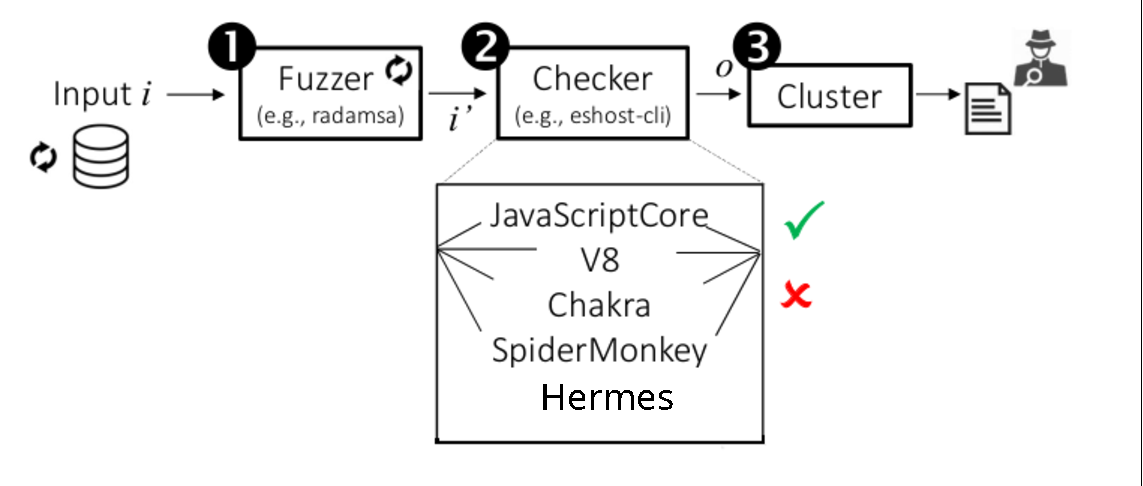
\includegraphics[trim=0 350 0 0,clip,width=1.0\textwidth]{diff-testing-runtimes}
  \vspace{-5ex}
  \caption{\label{fig:workflow}Differential Testing infrastructure overview.}
  \vspace{-2ex}
\end{figure}

\section{Cross-Engine Differential Testing}
\label{sec:design}

This section describes the infrastructure we used for cross-engine
differential testing. Figure~\ref{fig:workflow} illustrates the
workflow of the approach. It takes on input a list of JS files and
generates warnings on output. Numbered boxes in the figure denote the
data processors and arrowed lines denote data flows. The cycle icons
indicate repetition--the leftmost icon indicates that each file in the
input list will be analyzed in separate whereas the rightmost icon
shows that a single file will be fuzzed multiple times.

The bug-finding process works as follows. For a given test input, the
toolchain produces new inputs using some off-the-shelf input fuzzer
(step 1).  (Section~\ref{sec:objects:fuzzers} describes the fuzzers we
selected.)  Then, the oracle checks whether or not the output produced
for the fuzzed file is consistent across all engines (step 2). In case
the test passes in all engines or fails in all engines (\ie{}, the
output is consistent), the infrastructure ignores the
input. Otherwise, it considers the input as potentially
fault-revealing; hence, interesting for human inspection. Finally, to
facilitate the human inspection process, the infrastructure
prioritizes warnings and clusters them in groups (step 3). We describe
these features in Sections~\ref{sec:prioritization} and
\ref{sec:clusterization}. Note that a number of reasons exist, other
than a bug, to explain discrepancy (see
Tables~\ref{fig:piecharts-transplantation} and
~\ref{tab:false-positives}) and there is no clear automatic approach
to precisely distinguish false and true positives. As such, a human
needs to inspect the warning to classify the issue. As mentioned
earlier, this justifies why differential testing is challenging to
automate at the functional level.

For step 2, we considered using the open-source tool
eshost-cli~\cite{eshost-cli}, also used at Microsoft, for checking
output discrepancy. However, we noticed that eshost-cli does not
handle discrepancies involving crashes. As such, we forked the
eshost-cli GitHub project and implemented that functionality on it. It
is also important to note that our checker does not support the case
where the test fails in all engines but the kind of failure (\eg{},
exception thrown) is different. Currently, our infrastructure does not
report discrepancy for that case. For that, it would be necessary to
properly parse the error message to retrieve the error types. We left
that as future work as we already found several discrepancies even
without that.

%% \Mar{any difference in
%%   output is considered for reporting? are there any
%%   filtering?}\Igor{acho que nos equivocamos ao deixar o "eshost-cli",
%%   nao estamos mais utilizando isso devido a essa ferramenta nao
%%   capturar certos tipo de issues (e.g. crash), retirar tambem da Figura 2.
%%   A respeito de filtros nos reports, nao. Nos so capturamos o output,
%%   o que modificamos eh apenas a formatacao do output para coletar apenas a
%%   mensagem e nao o stack trace.
%%   }


\subsection{Prioritization}
\label{sec:prioritization}

We prioritized warnings based on their types, reflecting likelihood of
manifesting a real bug. We defined two types---``\hi{}'' and
``\lo{}''.

Warnings of the kind ``\hi{}'' are associated with the cases where the
test code executes without violating any internal checks, but it
violates an assertion declared in the test itself or its harness. The
rationale is that the test data is more likely to be valid in this
case as execution does not raise exceptions in application
code. Warnings of kind ``lo'' cover the remaining cases. These
warnings are more likely to be associated with invalid inputs. They
reflect the cases where the anomaly is observed during the execution
of application functions as opposed to assertions. We observed that
different engines often check pre-conditions of functions
differently. It can happen, for example, that one engine enforces a
weaker pre-condition, compared to another engine, on the inputs of a
function and that is acceptable.\Comment{ For instance, it is
  acceptable to pass values greater than \Fix{x} to function
  \CodeIn{\Fix{WWW}} in \Fix{y} but not in \Fix{z}.} In those cases,
the infrastructure would report a warning that is more likely to be
associated with an invalid input produced by the fuzzer, \ie{}, it is
likely to be a ``bug'' in the test code as opposed to a bug in the
engine. Recall that, for differential testing, we only use seed tests
that pass in all engines.

Despite the problem mentioned above, ``\lo'' warnings can reveal bugs.
Figure~\ref{fig:lo-truepositive} shows one of these cases. In this
example, the test instantiates an \CodeIn{ArrayBuffer} object and
stores an 8-bit integer at the 0 position. According to the
specification~\cite{ecmas262-getviewvalue}, a \CodeIn{RangeError}
exception should be thrown if a negative value is passed to the
function \CodeIn{ToIndex}, indirectly called by the test case from the
function call \CodeIn{getInt8()}. In this case, however, the \chakra{}
engine did not throw any exception, as can be confirmed from the
report that our infrastructure produces starting with text ``Engine
Messages'' at the bottom of Figure~\ref{fig:lo-truepositive}. This is
a case of undocumented precondition. It was fixed by
\chakra\ developers and is no longer present in the most recent
release of \chakra.

\subsection{Clusterization}
\label{sec:clusterization}

%% Prioritization helps to steer our focus to the warnings more likely to
%% reveal bugs, but there could be several tests producing similar
%% warnings.

Clusterization is complementary to prioritization; it helps to group
similar warnings reported by our infrastructure. We only clustered
``\lo'' warnings as ``\hi'' warnings produce messages that arise from
the test case, which are typically distinct.

\Fix{Figure~\ref{fig:lo-truepositive} shows a test was originally
available in the \jsc codebase.  The \radamsa fuzzing technique
mutated the test. In particular, it introduced the negative
long \texttt{-1770523502845470856} as a parameter of the
\texttt{view.getInt8()} method. Before the mutation, the
\texttt{view.getInt8()} method received a zero integer.}
At the botom of this figure, there is a sequence of
three elements that we use to characterize a warning--1) the
identifier of an engine, 2) the exception it raises, and 3) the
message it produces on a ``\lo'' warning.  This sequence of triples
defines a warning signature that we use for clustering. It is worth
mentioning that we filter references to code in messages as to
increase ability to aggregate warnings. Any warnings, including this
one, that has this same signature will be included in the same
``bucket''. Considering the example from
Figure~\ref{fig:lo-truepositive}, the signature for that cluster will
be [(JavaScriptCore, ``RangeError'', ``byteOffset cannot be
  negative''), (SpiderMonkey, ``RangeError'', ``invalid or
  out-of-range index''), (V8, ``RangeError'', ``Offset is outside the
  bounds of the DataView'')].

\begin{figure}[t!]
  \centering
  \begin{lstlisting}
var buffer = new ArrayBuffer(64);
var view = new DataView(buffer);
view.setInt8(0,0x80);
assert(view.getInt8(-1770523502845470856) === -0x80);

Engines Messages (1:V8, 2:JavaScriptCore, 3:SpiderMonkey):
1. RangeError: Offset is outside the bounds of the DataView
2. RangeError: byteOffset cannot be negative
3. RangeError: invalid or out-of-range index
  \end{lstlisting}
  \caption{\label{fig:lo-truepositive}Example of a ``\lo'' warning
    that led to a confirmed bug report in \chakra. The bug is caused
    by a required precondition check in the implementation of function
    \CodeIn{ToIndex}~\cite{ecmas262-getviewvalue}, which is indirectly called by the test. }
\end{figure}

\subsection{Fuzzers}
\label{sec:objects:fuzzers}

Fuzzers are typically categorized in two main groups--those that build
inputs anew (generational) and those that modify existing inputs
(mutational). We used two black-box mutational
fuzzers\Comment{Radamsa~\cite{radamsa} and QuickFuzz~\cite{quickfuzz}}
in this study. In the following, we provide rationale for this
selection.

Generational fuzzers are typically grammar-based. These fuzzers
generate a new file using the grammar of the language whose inputs
should be fuzzed. Intuitively, those fuzzers implement a traversal of
the production rules of the input grammar to create syntax trees,
which are then pretty-printed. Consequently, this approach produces
inputs that are syntactically valid by construction. We analyzed four
grammar-based fuzzers--Grammarinator~\cite{grammarinator},
jsfunfuzz~\cite{jsfunfuzz},
LangFuzz~\cite{Holler:2012:FCF:2362793.2362831}, and
Megadeth~\cite{grieco2016quickfuzz}.  Unfortunately, none of those
were effective out of the box. For example, we produced 100K inputs
with Grammarinator and only few inputs were valid. With Megadeth, we
were able to produce more\Comment{ \Fix{Y, Y$>$Y?}} valid inputs as it
contains some heuristics to circumvent violations of certain typing
rules.\Comment{ such as \Fix{variable used must be defined?}.}
Nonetheless, running those inputs in our infrastructure we were unable
to find discrepancies. Inspecting those inputs, we realized that they
reflected very simple scenarios. To sum up, a high percentage of inputs
that Grammarinator and Megadeth generated were semantically-invalid
that we needed to discard whereas the valid inputs manifested no
discrepancies. Considering jsfunfuzz~\cite{jsfunfuzz}, we noticed
that, in addition to the issues mentioned above, it produces inputs
that use functions that are only available in the \smonkey{}
engine. We would need either to mock those functions in other engines
or to discard those tests. Considering
LangFuzz~\cite{Holler:2012:FCF:2362793.2362831}, the tool is not
publicly available. Another fundamental issue associated with
generational fuzzers in our context is that the tests they produce do
not contain assertions; to enable the integration of this kind of
fuzzers in our infrastructure---we would need to look for
discrepancies across compiler error messages as opposed to assertion
violations.  All in all, although grammar-based fuzzers have been
shown effective to find real
bugs~\cite{Holler:2012:FCF:2362793.2362831}, we did not consider those
fuzzers in this study for the reasons above.

%% Our
%% infrastructure supports any grammar fuzzer with a few
%% adjusts. However, we try to integrate several grammar-based fuzzers,
%% for example
%% and \Fix{others fuzzers} to
%% generate new JavaScript files based on grammar, but after several runs
%% it was observed that this approach was ineffective due the amount of
%% invalid files and/or files without discrepancies.
%% For example, if we
%% ran Grammarinator to generate 1K JS files ten times with a random seed
%% generation, we obtained \Fix{XX\%} of valid files. Checking in our
%% environment almost \Fix{XX\%} are js files that shows undefined
%% variables and due the differential testing in our environment all
%% engines will raise a SyntaxError and this approach was not relevant to
%% our experiment.

%% We initially considered used representatives of popular fuzzing approaches. For
%% random-based fuzzing we used Radamsa~\cite{radamsa}; for
%% coverage-based fuzzing we used
%% \Fix{AFL~\cite{afl}/libfuzzer~\cite{libfuzzer}?}, and for
%% generative-based fuzzing we used
%% \Fix{grammarinator,jsfunfuzz?}. Details on how these fuzzers work can
%% be found elsewhere~\cite{fuzz-bart}.

Mutational fuzzers can be either white-box or black-box. White-box
mutational fuzzers are typically coverage-based. American Fuzz Loop
(AFL)~\cite{afl} and libFuzzer~\cite{libfuzzer} are examples of this
kind of fuzzers. These fuzzers run tests inputs against instrumented
versions of the program under testing with the typical goal of finding
universal errors like crashes and buffer overflows. The instrumentation
adds code to collect branch coverage and to monitor specific
properties\footnote{There are options in the clang toolchain to build
  programs with fuzzing instrumentation~\cite{libfuzzer}. clang
  provides several sanitizers for property
  checking~\cite{clang-documentation}.}. AFL uses coverage to determine
inputs that uncover a new branch and hence should be fuzzed more
whereas libFuzzer uses evolutionary generation--it tries to minimize
the distances to still-uncovered branches of the program. AFL takes
the instrumented program binary (say, a JS engine) and one seed input
to that program (say, a JS program) and produces on output
fault-revealing inputs, if found. Considering our context of
application, we needed to instrument one runtime engine for fuzzing.
We chose \veight\ for that. Unfortunately, we found that most of the inputs produced
by AFL violate the JS grammar. Furthermore, the fuzzing task can take
days for a single seed input and there is no simple way to guide the
exploration\footnote{Exchanged emails with the tool author.}. That
happens because the fuzzer aims to explore the entire decision tree
induced from the engine's main function, including the branches
associated with the higher layers of the compiler (\eg{}, lexer and
parser). It is worth mentioning that Google mitigates that problem
with libFuzzer by asking developers to create fuzz targets for
specific program
functions~\cite{libFuzzer-tutorial-google,libFuzzer-chromium-google}. Although
that approach has shown to be effective, it requires domain knowledge
to create the calling context to invoke the fuzz target. For that, we
decide not to consider coverage-based in this study.

We used two black-box mutational fuzzers in this
study--\radamsa~\cite{radamsa} and \quickfuzz~\cite{quickfuzz}. These
fuzzers require no instrumentation and domain-knowledge. They mutate
existing inputs randomly. The strength of the approach is
limited by the quality of the test suite and the supported mutation
operators, which are typically simple. We chose these specific fuzzers
because, conceptually, one complements the other. \quickfuzz\ creates
mutations like \radamsa. However, in contrast to \radamsa, \quickfuzz\ is aware
of the \js\ syntax; it is able to replace sub-trees of the syntax
tree~\cite{grieco2016quickfuzz} with trees created anew.

\section{Results}
\label{sec:results}

The goal of this paper is to assess ability of
test transplantation and differential testing
to find functional bugs
in \javascript\ engines. Based on that, we pose three questions:
\begin{description}[leftmargin=.5in]
\item[RQ1.] How conformant are the engines to the Test262 suite?
\item[RQ2.] How effective is test transplantation to find bugs?
\item[RQ3.] How effective is cross-engine differential testing to find bugs?
\end{description}

The first question focuses on the conformance of our selected engines
to the official Test262 suite~\cite{ecma262-conformance-suite}
(Section~\ref{sec:stability}). In the limit, bugs would have low
relevance if the engines are too unreliable. The second question
focuses on the effectiveness of test transplantation
(Section~\ref{sec:transplantation}). The rationale for using inputs
from different engines is that developers consider different goals
when writing tests---suites written for a given engine may cover
scenarios not covered by a different engine. The third question
evaluates the effectiveness of cross-engine differential testing to
find bugs (Section~\ref{sec:cross-engine-diff-testing-results}). The
rationale for this question is that fuzzing inputs may explore
scenarios not well-tested by at least one of the engines.

\subsection{Answering RQ1 (Conformance)}
\label{sec:stability}

The ECMA Test262~\cite{ecma262-conformance-suite} test suite serves to
check conformance of engines to the \js\ standard. It is
acceptable to release engines fulfilling the specification only
partially~\cite{kangax}. We expect that the pass rate on this suite
provide some indication of the engine's maturity. In the limit, it is
not desirable to flood bug reports on engines at early stages of
development.
\Fix{For this experiment, we ran the suite once a day for seven consecutive
days and averaged the passing ratios.
We performed seven consecutive executions because,
since the studied JS engines release new versions on a daily basis,
we wanted to make sure if the failing tests raised by the Test262 suite
were rapidly fixed by the maintenance team. If these errors were quickly
fixed, that would suggest that this given engine would be aligned with
the ECMAScript specification.}
Table~\ref{tab:test262} shows
the average number of passing tests over this period. The variance of
results was negligible; for that reason, we omitted standard
deviations. We noticed that all four engines but \chakra{} used some
variant of the Test262 suite as part of their regression process, but
we used the same version in this
experiment~\cite{ecma262-conformance-suite}.

\begin{table}
  %\vspace{-4ex}
  \centering
  \caption{\label{tab:test262}Percentage of passing tests on
    the Test262 conformance suite.}
  %\small
  \begin{tabular}{rr}
    \toprule
    engine & \% passing \\
    \midrule
    \jsc & \percentSuiteTestJSC{}\\
    \veight{} & \percentSuiteTestVeight{} \\
    \chakra{} & \percentSuiteTestChakra{} \\
    \smonkey{} & \percentSuiteTestSM{} \\
    \hermes & \percentSuiteTestHermes{} \\
    \bottomrule
  \end{tabular}
  %\normalsize
\end{table}

%Nao envolver o hermes nos experimentos antigos pq o hermes vai
%lancar erros pq a funcionalidade não foi implementada

Results show that there are still many unsupported scenarios as can be observed from the
percentages in the table. The number of passing tests is high and
similar for \jsc, \veight{}, and \smonkey\ whereas \hermes performs
worse when compared to the other engines.
\Fix{This happens because \hermes
still has many unsupported features, such as Proxy, Promisse, and Async.}
Moreover, one can also note that \chakra\ also a low passing ratio
in this test suite and the one we were able to find more bugs (as per
Figure~\ref{fig:summary}). Although it is plausible to find
correlation between the passing ratios and reliability as measured by
the number of bugs found, we do not imply causality. As aforementioned,
it is important
to note that failures in this conformance test suite indicates missing
features as opposed to bugs.

\begin{center}
  \fbox{
    \begin{minipage}{8cm}
      \textit{Summary:}~Most of the engines seem to adhere well to the
      \js\ standard. Except for \hermes and \chakra, the passing ratio of all
      engines is above 90\%.
      \end{minipage}
    }
\end{center}


\subsection{Answering RQ2 (Test Transplantation)}
\label{sec:transplantation}

This section reports results of test transplantation. More
specifically, we analyzed the failures observed when running a test
suite original from a given engine in another engine. Intuitively, we
want to assess how effective is the idea of cross-fertilization of
testing knowledge among \js\ developers.

%\vspace{0.5ex}
\subsubsection{Methodology}
\label{sec:methodology}
In this experiment, a developer with experience in \js\ analyzed each
test failure, affecting a particular engine, and classified that
failure as potentially fault-revealing or not. The authors supervised
the classification process to validate correctness. For the
potentially fault-revealing cases, one of the authors inspected the
scenario and, if agreed on the classification, reported the bug to the
issue tracker of the affected engine.

\begin{table}[t]
  \small
  \centering
  \caption{\label{tab:cross-testing}Number of failures with
    Test Transplantation.}
  \renewcommand*{\arraystretch}{0.9}
  \begin{tabular}{crrrrr}
    \toprule
    test suite\textbackslash{}engine & \jsc & \veight{} & \smonkey{} & \chakra{} & \hermes{} \\
    \midrule
    % \Fix{Versions (03.08)} & 234555 & 7.0.158 & 62.0b14 & 1.10.1 \\
    \Comment{
      Lembrar dos testes que os testes da propria engine falham:
      V8 0
      JSC 2
      Spidermonkey 58
    }
    \jsc & - & 10 & 10 & 59 & 340  \\
    \veight{} & 41 & - & 3 & 5 & 315 \\
%    \chakra{} & - & - & - & -  \\
    \smonkey{} & 218 & 107 & - & 281 & - \\
    Hermes & 8 & 14 & 8 & 26 & -  \\
    Duktape & 0 & 4 & 4 & 1 & 140  \\
    \jerry{} & 23 & 25 & 22 & 23 & 311  \\
    JSI & 0 & 0 & 0 & 0 & 40\\
   Tiny-js & 0 & 0 & 0 & 0 & 10  \\
    \midrule
   \textbf{total} & 290 & 160 & 47 & 395 & 1156 \\
    \bottomrule
  \end{tabular}
  \vspace{-3ex}
\end{table}

\subsubsection{Results}
\label{sec:results}

Table~\ref{tab:cross-testing} shows the number of failures observed
for each pair of test suite and engine. The first column shows the
test suites and the first row shows the engines that run those
tests. We use a dash (``-'') to indicate that we did not consider the
combinations that associate a test suite with its parent engine.
\Fix{
In particular, we were not able to reuse the \smonkey tests on the
\hermes engine. This happened because \smonkey has its own assertion
framework, but \hermes did not interpret these assertions, resulting
in failures in all test executions from this engine. These failures
did not happen when the \smonkey tests were transplanted to the other engines,
though.
}
failures in those cases would either indicate regressions or flaky
tests as opposed to unknown bugs for that engine. As explained in
Section~\ref{sec:seeds}, we used in this experiment the
\totalTestFilesForTestTransplantation{} tests included in the
rectangle area under column ``type-in-all'' from
Table~\ref{tab:test-suites}. Running those tests we observed a total
of \failuresTestTrans{} failures manifested across
\failuresTestTransDistictFiles{} distinct files
(\failuresTestTransPercent{} of total).  Table~\ref{tab:cross-testing}
shows that \smonkey\ was the engine that failed the least whereas
\chakra\ was the engine that failed the most. The \smonkey\ test suite
also revealed more failures than any other, as expected, given
that it is the suite with more tests (see
Table~\ref{tab:test-suites}).


%%  As another example, some tests from \Fix{Y} use the
%% implementation-dependent description message\Mar{what is the name of
%%   the property?} encapsulated in an \CodeIn{Error} object in
%% assertions. As such, those tests fail in all engines but
%% \Fix{Y}.

\sloppy The sources of false positives found in this experiment are as
follows: \textbf{Undefined Behavior.} False positives of this kind are
manifested when tests cover implementation-dependent behavior, as
defined in the ECMA262 specification~\cite{ecmas262-spec}. For
example, one of the tests from \jerry\ uses the function
\CodeIn{Number.toPrecision([precision])}, which translates a number to
a string, considering a given number of significant digits. The
floating-point approximation of the real value is
implementation-dependent, making that test to pass only in
\chakra. \textbf{Timeout/OME\footnote{ome is for out of memory
    error.}.} False positives of this kind typically manifest when the
engine that runs the test does not optimize the code as the original
engine of the test. As result, the test fails to finish at the
specified time budget or it exceeds the memory budget. For example, a
test case from \jsc defines a function with a tail-call
recursion. The test fails in all engines but \jsc, which implements
tail-call optimization. \textbf{Not implemented.} False positives of
this kind manifest when a test fails because it covers a function that
is part of the official spec, but is not implemented in the target
engine yet. For example, at the time of writing, \chakra{} did not
implement by default various properties from the \mcodeid{Symbol}
object. These properties are only available activating the ES6
experimental mode with the flag \CodeIn{-ES6Experimental}.
\textbf{Non-Standard Element.} These cases manifest when a function or
an object property is undefined in the execution engine but we were
unable to capture that by looking for error types like
\CodeIn{ReferenceError} and \CodeIn{TypeError}.\Comment{ For example,
  we found cases where the test (or its harness) fails in an assertion
  because of an undefined property.}  \textbf{Other.} This category
includes other sources of false positives. For example, it includes
the cases where the test was valid for some previous version of the
spec but is no longer valid for the current spec.

\begin{table}
  \centering
  \caption{\label{fig:falsepositives}\label{fig:truepositives}\label{fig:piecharts-transplantation}Distribution
    of False (FP) and True Positives (TP).}
  %\setlength{\tabcolsep}{3pt}
  \renewcommand*{\arraystretch}{0.9}
  \begin{tabular}{ccr}
    \toprule
    & source &  \#\\
    \midrule
    \multirow{5}{*}{FP} & Undefined Behavior & \noTransUndefined{} \\
    & Timeout/OME & \noTransTimeout{} \\
    & Not Implemented & \noTransNotImplemented{} \\
    & Non-Standard Element & \noTransNonStandard{} \\
    & Other & \noTransOther{} \\
    \midrule
    \multirow{2}{*}{TP} & Duplicate & \noTransTPDuplicated{} \\
    & Bug & \noTransTPBugs{} \\
    \bottomrule
  \end{tabular}
\end{table}

Table~\ref{fig:piecharts-transplantation} shows the distribution of
False Positives (FPs) and True Positives (TPs). The sum of the numbers
in this table correspond to the number of files that manifested
failures, \ie{}, \failuresTestTransDistictFiles{}. Considering false
positives, ``Undefined Behavior'' was the most predominant
source. Considering true positives, we found a reasonable number of
duplicate reports, but not high enough to justify attempting to
automate the detection of duplicates.

\begin{table}[t!]
  %\small
%  \setlength{\tabcolsep}{5pt}
  \renewcommand{\arraystretch}{0.9}
  %  \vspace{-3ex}
    %  \scriptsize
      \centering
      \caption{List of bugs reports from Test Transplantation.}
      \label{tab:test-transplantation-bugs}

      \begin{tabular}{rccccc}

        \toprule \# & Engine  & Version & Status & Severity & Suite \\
        \midrule
       1  & \jsc{} & 606.1.9.4 & New  & - & \jerry{} \\
       2  & \chakra{}  & 1.9 & \textbf{Confirmed} & 2 & \smonkey{} \\
       3  & \chakra{}  & 1.9 & \textbf{Fixed}   & 2 & \smonkey{} \\
%      \midrule
       4  & \chakra{} & 1.10-beta & \textbf{Confirmed} & 2 & \smonkey{} \\
       5  & \jsc{} & 606.1.9.4 & New &  -  & \smonkey{}\\
%      \midrule
       6  & \jsc{} & 606.1.9.4 & New & - & \smonkey{} \\
       7  & \jsc{} & 606.1.9.4 & \textbf{Fixed} & 2 & \smonkey{}\\ % webkit
       8  & \chakra{} & 1.10-beta & \textbf{Fixed} & 3 & \smonkey{}\\
       9  & \chakra{} & 1.10-beta & \textbf{Fixed} & 2 & \jsc{}\\
       10 & \chakra{} & 1.10-beta & \textbf{Fixed} & 2 & \smonkey{}\\
       11 & \chakra{} & 1.11-beta & \textbf{Fixed} & 2 & \jsc{}\\
       12 & \chakra{} & 1.11-beta & \textbf{Confirmed} & 2 & \jerry{}\\ % duktape
       13 & \chakra{} & 1.10.1 & \textbf{Fixed} & 2 & \smonkey{}\\
       14 & \jsc{} & 233840 & Duplicated & 2 & \jerry{}\\
       15 & \chakra{} & 1.10.1 & \textbf{Fixed} & 2 & \jerry{}\\ % test262
       16 & \chakra{} & 1.10.1 & \textbf{Fixed} & 3 & \jerry{}\\
       17 & \jsc{} & 234555 &\textbf{Fixed} & 2 & \jerry{}\\
       18 & \chakra{} & 1.10.1 & \textbf{Fixed} & 3 & \jerry{}\\
       19 & \jsc{} & 234654 & \textbf{Fixed} & 2 & \jerry{}\\
       20 & \veight{} & 7.0.181 & \textbf{Fixed} & 3 & \jerry{}\\
       21 & \jsc{} & 234689 & New & - & \jerry{}\\
       22 & \veight{} & 7.0.237 & WontFix & 2 & Duktape\\
       23 & \chakra{} & 1.10.2 & \textbf{Fixed} & 2 & \smonkey{}\\
       24 & \jsc{} & 235121 & \textbf{Fixed} & 2 & \smonkey{}\\
       25 & \jsc{} & 235121 & \textbf{Fixed} & 2 & \smonkey{}\\
       26 & \veight{} & 7.0.244 & \textbf{Fixed} &  2  & \smonkey{}\\
       27 & \chakra{} & 1.10.2 & \textbf{Fixed} &  2  & \smonkey{}\\
       28 & \jsc{} & 235121 & New & - & \smonkey{}\\
       29 & \chakra & 1.11.19 & \textbf{Confirmed}  & - & \babel \\
       30 & \jsc & 262693 & New & - & \babel \\
       31 & \jsc    & 262693 & New & - & \babel \\
       32 & \smonkey & 77.0b9 & \textbf{Fixed} & 3 & \hermes\\
       %33 & \hermes & 0.5.0 & WontFix & - & \babel \\
       %34 & \hermes & 0.5.0 & \textbf{Confirmed} & - & \babel \\
       %35 & \hermes & 0.5.0 & WontFix  & - & \babel \\
       \bottomrule
      \end{tabular}
      \vspace{-2ex}
\end{table}

% JavaScript-C77.0 (77.0b9)
% tracking urls
% 1  & 4/18  & \jsc{} & 606.1.9.4 & New  & \href{https://bugs.webkit.org/show\_bug.cgi?id=184749}{\#184749} & - & \jerry{} \\
% 2  & 4/23 & \chakra{}  & 1.9 & \textbf{Confirmed}  & \href{\repoCH/issues/5033}{\#5033} & 2 & \smonkey{} \\
% 3  & 4/29 & \chakra{}  & 1.9 & \textbf{Fixed}   & \href{\repoCH/issues/5065}{\#5065} & 2 & \smonkey{} \\
% 4  & \multirow{2}{*}{4/29} & \chakra{} & 1.10-beta & \textbf{Confirmed} & \href{\repoCH/issues/5067}{\#5067} & 2 & \smonkey{} \\
% 5  &  & \jsc{} & 606.1.9.4 & New & \href{https://bugs.webkit.org/show\_bug.cgi?id=185130}{\#185130} &  -  & \smonkey{}\\
% 6 & 5/02  & \jsc{} & 606.1.9.4 & New  & \href{https://bugs.webkit.org/show\_bug.cgi?id=185208}{\#185208} & - & \smonkey{} \\
% 7 & \multirow{2}{*}{5/02}  & \jsc{} & 606.1.9.4 & \textbf{Fixed} & \href{https://bugs.webkit.org/show_bug.cgi?id=185211}{\#185211} & 2 & \smonkey{}\\ % webkit
% 8 &  & \chakra{} & 1.10-beta & \textbf{Fixed} & \href{\repoCH/issues/5087}{\#5087} & 3 & \smonkey{}\\
% 9 & 5/17  & \chakra{} & 1.10-beta & \textbf{Fixed} & \href{\repoCH/issues/5187}{\#5187} & 2 & \jsc{}\\
% 10 & 5/21  & \chakra{} & 1.10-beta & \textbf{Fixed} & \href{\repoCH/issues/5203}{\#5203} & 2 & \smonkey{}\\
% 11 & 6/28  & \chakra{} & 1.11-beta & \textbf{Fixed}  & \href{\repoCH/issues/5388}{\#5388} & 2 & \jsc{}\\
% 12 & 7/10  & \chakra{} & 1.11-beta & \textbf{Confirmed} & \href{\repoCH/issues/5442}{\#5442} & 2 & \jerry{}\\ % duktape
% 13 & 7/18  & \chakra{} & 1.10.1 & \textbf{Fixed} & \href{\repoCH/issues/5478}{\#5478} & 2 & \smonkey{}\\
% 14 & 7/18  & \jsc{} & 233840 & Duplicated & \href{https://bugs.webkit.org/show_bug.cgi?id=187777}{\#187777} & 2 & \jerry{}\\
% 15 & 7/18  & \chakra{} & 1.10.1 & \textbf{Fixed} & \href{\repoCH/issues/5549}{\#5549} & 2 & \jerry{}\\ % test262
% 16 & 8/07  & \chakra{} & 1.10.1 & \textbf{Fixed} & \href{\repoCH/issues/5576}{\#5576} & 3 & \jerry{}\\
% 17 & 8/07  & \jsc{} & 234555 &\textbf{Fixed} & \href{https://bugs.webkit.org/show_bug.cgi?id=188378}{\#188378} & 2 & \jerry{}\\
% 18 & 8/07  & \chakra{} & 1.10.1 & \textbf{Fixed} & \href{\repoCH/issues/5579}{\#5579} & 3 & \jerry{}\\
% 19 & 8/07  & \jsc{} & 234654 & \textbf{Fixed} & \href{https://bugs.webkit.org/show_bug.cgi?id=188382}{\#188382} & 2 & \jerry{}\\
% 20 & 8/08  & \veight{} & 7.0.181 & \textbf{Fixed} & \href{https://bugs.chromium.org/p/v8/issues/detail?id=8033}{\#8033} & 3 & \jerry{}\\
% 21 & 8/08  & \jsc{} & 234689 & New & \href{https://bugs.webkit.org/show_bug.cgi?id=188407}{\#188407} & - & \jerry{}\\
% 22 & 8/16  & \veight{} & 7.0.237 & WontFix & \href{https://bugs.chromium.org/p/v8/issues/detail?id=8064}{\#8064} & 2 & Duktape\\
% 23 & 8/22  & \chakra{} & 1.10.2 & \textbf{Fixed} & \href{\repoCH/issues/5621}{\#5621} & 2 & \smonkey{}\\
% 24 & 8/22  & \jsc{} & 235121 & \textbf{Fixed} & \href{https://bugs.webkit.org/show_bug.cgi?id=188874}{\#188874} & 2 & \smonkey{}\\
% 25 & \multirow{3}{*}{8/22} & \jsc{} & 235121 & \textbf{Fixed} & \href{https://bugs.webkit.org/show_bug.cgi?id=188875}{\#188875} & 2 & \smonkey{}\\
% 26 &  & \veight{} & 7.0.244 & \textbf{Fixed} & \href{https://bugs.chromium.org/p/v8/issues/detail?id=8082}{\#8082} &  2  & \smonkey{}\\
% 27 &  & \chakra{} & 1.10.2 & \textbf{Fixed} & \href{\repoCH/issues/5624}{\#5624} &  2  & \smonkey{}\\
% 28 & 8/23  & \jsc{} & 235121 & New & \href{https://bugs.webkit.org/show_bug.cgi?id=188877}{\#188877} & - & \smonkey{}\\



Table~\ref{tab:test-transplantation-bugs} lists all bugs we found with
test transplantation. The first column shows the identifier we
assigned to the bug\Comment{, column ``Date'' shows the date the bug
  was reported in the format ``m/dd'',}, column ``Engine'' shows the
affected engine, column ``Status'' shows the status of the bug report
at the time of the writing. The status string appears in bold face for
status ``Confirmed'' or higher, \ie{}, ``Assigned'' and ``Fixed''.
Column ``Severity'' shows the severity of confirmed bugs, and,
finally, column ``Suite'' shows the name of the engine that originated
the test.  (We omitted the URLs of the issues to protect anonymity.)
Considering severity levels, we found that \jsc~\cite{jsc-severity}
and \smonkey{}~\cite{mozilla-severity} developers use five levels,
whereas \chakra{}~\cite{chakra-severity} and
\veight{}~\cite{v8-severity} developers use only three. As usual, the
smallest the severity value the highest the severity of the bug. We
use a dash (``-'') in place of the severity level for the cases where
the bug report is pending confirmation. Of the
\noBugsTransplantation{} bugs we reported in this experiment,
\noBugsTransplantationConfirmed\ were promoted from the status ``New''
to ``Confirmed''. Of these, \noBugsTransplantationSeverityTwo{} are severity-2 bugs.  Although we did
not find any critical bugs, most of the bugs are seemingly important
as per the categorization given by engineers. Analyzing the issue
tracker of \chakra, we found that severity-1 bugs are indeed
rare. Considering the number of bug reports confirmed by developers,
\chakra{} was the engine with the highest number--\bugsChakra{} (with \bugsChakraFixed{} bugs
fixed). Considering the remaining engines, \veight{} developers
confirmed the \noTransVeightBugsReported{} bugs we reported, fixing
\noTransVeightBugsFixed{}. Curiously, Google
engineers confirmed the issued bug reports in a few hours. Overall, we
found that development teams of other engines, specially \jsc\, took
much longer to analyze bug reports as can be observed in the
\jsc\ stacked bar from Figure~\ref{fig:stacked-engine}.
However, the bugs the \jsc team confirmed were quickly fixed.

%% Overall, we found these results promising given that precision (\ie{},
%% the ratio of true positives over all reports) needs to take into
%% account the cost of inspecting the failure~\cite{harman-ohearn-2018};
%% it took a week for the developer to inspect the entire set of
%% failures. The precision for \jsc\ was \Fix{X\%} (\ie, XX/270), which
%% seems a low rate, but it took approximately \Fix{x} days to find
%% \Fix{y} real bugs on this engine. Section~\ref{sec:bugs} shows samples
%% of false and true positives.

\begin{center}
  \fbox{
    \begin{minipage}{8cm}
      \textit{Summary:}~Test transplantation was effective at finding
      functional bugs. Although the cost of classifying failures was
      non-negligible, the approach revealed several non-trivial bugs
      in three of the four engines we analyzed.
      \end{minipage}
    }
\end{center}


\subsection{Answering RQ3 (Differential Testing)}
\label{sec:cross-engine-diff-testing-results}

This section reports the results obtained with cross-engine differential
testing. More precisely, we report results obtained by fuzzing test
inputs, running those inputs on different engines, and checking the
outcomes with a differential oracle.

\vspace{0.5ex}
\subsubsection{Methodology}
The experimental methodology we used is as follows. As explained in
Section~\ref{sec:objects:fuzzers}, we used Radamsa~\cite{radamsa} and
QuickFuzz~\cite{quickfuzz} for fuzzing. To avoid experimental noise,
we only fuzz test files that pass in all engines--a total of
\totalTestFilesPassInAll\ tests satisfy this restriction. Those tests
appear under the column ``no-fail-in-all'' on
Table~\ref{tab:test-suites}.  We want to avoid the scenario where
fuzzing produces a fault-revealing input based on a test that was
already revealing failures on some engine. This decision facilitates
our inspection task; it helps us establish cause-effect relationship
between fuzzing and the observation of discrepancy.  We configured our
infrastructure (see Figure~\ref{fig:workflow}) to produce 20
well-formed fuzzed files per input file, \ie{}, the number of fuzzing
iterations can exceed the number above as we discard generated files
that are syntactically invalid.

%%  That
%% finding would be important to reduce inspection cost and guide future
%% developments of this approach.

\vspace{0.5ex} \lbrack{}Exploratory Phase\rbrack{} For the first
three months of the study, our inspection process was exploratory.  In
this phase, we wanted to learn whether or not black-box fuzzers could
reveal real bugs and how effective was the \hi{}-\lo\ warning
classification.  We expected the number of warnings to increase
dramatically compared to the previous experiment and, if we realized
that the ratio of bugs from \lo\ warnings was rather low, we could
focus our inspection efforts on \hi\ warnings. To run this experiment,
we trained eight students in analyzing the warnings that our
infrastructure produces. The students were enrolled in a
graduate-level testing class. We listed warnings in a spreadsheet and
requested the students to update an ``owner'' column indicating who
was working on it, but we did not enforce a strict order on the
warnings the students should inspect. Recall from
Section~\ref{sec:clusterization} that we clustered \lo\ warnings in
buckets. For that reason, we only listed one \lo\ warning per
representative class/bucket in the spreadsheet. First, we explained,
through examples, the possible sources of false alarms they could find
and then we asked the students to use the following procedure when
finding a suspicious warning. Analyze the parts of the spec related to
the problem and, if still suspicious, look for potential duplicates on
the bug tracker of the affected engine using related keywords. If none
was reported, indicate in the spreadsheet that that warning is
potentially fault-revealing. We encouraged students to use
lithium~\cite{lithium} to minimize long test cases\Comment{; the tests
  from the Mozilla suite are often longer than others}. A bug report
was filed only after one of the authors reviewed the diagnosis. Each
student found at least one bug using this methodology.

\vspace{0.5ex}
\lbrack{}Non-Exploratory Phase\rbrack{} Results obtained in the
exploratory phase confirmed our expectations that most of the bugs
found during the initial period of investigation were related to
\hi\ warnings. For that reason, we changed our inspection
strategy. This time, only the co-authors inspected the bugs using a
similar discipline as before. However, the set of warnings inspected
and the order of inspection changed. We restricted our analysis to
\hi\ warnings and, aware that we would be unable to analyze each and
every warning reported, we grouped those warnings per engine,
analyzing each group in a round-robin fashion.  At each iteration, we
analyzed \warningsIteration{} warnings in each group. A warning
belongs to the group of a given engine if only that engine manifests
distinct behavior, \ie{}, it produces a distinct output compared to
others. We separated in a distinct group the warnings for which two
engines diverge. The rationale for this methodology was to give
attention to each engine more uniformly, enabling more fair comparison
across engines.

%% Table~\ref{tab:summary-lo}
%% shows statistics of \lo\ warnings obtained when fuzzing inputs with
%% different tools. Column ``\# buckets'' shows the number of buckets
%% associated with ``\lo'' warnings, column ``\# files'' shows the total
%% number of files involved in these warnings, and column ``avg. \# files
%% per bucket'' shows the average number of files per bucket. Note that,
%% although the number of buckets and files differ substantially across
%% fuzzers, the difference of files per bucket was not very high.\Mar{not
%% sure how relevant is this par.}

%% \begin{table}[t]
%%   \small
%%   \centering
%%   \caption{\label{tab:summary-lo}Summary of \lo\ warning reports.}
%%   \begin{tabular}{crrr}
%%     \toprule
%%     & \# buckets & \# files & avg. \# files per bucket \\
%%     \midrule
%%     \radamsa{} & 82 & 319 & 3.8 \\
%%     \quickfuzz{} & 78 & 218 & 2.7 \\
%%     \bottomrule
%%   \end{tabular}
%% \end{table}

\vspace{0.5ex}
\subsubsection{Results}~Table~\ref{tab:summary-hi} shows statistics of \hi\ warnings. The table breaks down \hi\ warning by the affected
engine, \ie, the engine manifesting distinct output among those
analyzed. Column ``+1'' shows the cases where more than one engine
disagree on the output. Note from the totals that the ordering of
engines is consistent with the one observed on
Table~\ref{tab:cross-testing}, with \chakra\ and \jsc\ in first and
second places, respectively, in number of warnings.


\begin{table}[t]
  \small
  \setlength{\tabcolsep}{4.5pt}
  \centering
  \caption{\label{tab:summary-hi}Number of \hi\ warning
    reports per engine.}
  \begin{tabular}{crrrrr}
    \toprule
    fuzzer\textbackslash{}engine & \jsc\ & \veight\ & \chakra & \smonkey & +1\\
    \midrule
    \radamsa{} & 151 & 50 & 331 & 94 & 528 \\ % 137 & 47 & 323 & 21 & 483
    \quickfuzz{} & 83 & 63 & 351 & 21 & 403 \\ % 81 & 62 & 349 & 13 & 369
    \midrule
    \textbf{total} & 234 & 113 & 682 & 115 & 931 \\ % 218 & 109 & 672 & 34 & 852
    \bottomrule
  \end{tabular}
\end{table}


Table~\ref{tab:false-positives} shows the distribution of false
positives per source. The sources of imprecision are as defined in
Section~\ref{sec:transplantation} with the addition of two new
sources, which we did not observe before. These new sources are
marked with a ``*'' in the table. The source ``Invalid Input''
indicates that the test input violated some part of the
specification. For example, the test indirectly invoked some function
with unexpected arguments; this happens because fuzzing is not
sensitive to function specifications. Consequently, it can replace
valid with invalid inputs. The source ``Error Message Mismatch''
corresponds to the cases where the fuzzer modifies the assertion
expression (\eg{}, some string expression or regular expression).

\begin{table}[t]
  \small
  \centering
  \caption{\label{tab:false-positives}Distribution of False (FP)
    and True Positives (TP).}
  \begin{tabular}{ccrr}
    \toprule
    & & \radamsa\ & \quickfuzz\ \\
    \midrule
    \multirow{4}{*}{FP} & Undefined Behavior & 42 & 16 \\ % 26 & 9
    & Timeout/OME & 30 & 15 \\ % 28 & 13
    & * Invalid Input & 46 & 55 \\ % 39 & 48
    & * Error Message Mismatch & 41 & 12 \\ % 41 & 12
    \midrule
    \multirow{2}{*}{TP} & Duplicate & 36 & 28\\ % 34 & 28
    & Bug & 15 & 7\\
    \bottomrule
  \end{tabular}
\end{table}

%% \Igor{devemos remover isso da
%% etapa de fuzzing upcoming feature falha mesmo sem fuzzing...$\rightarrow$
%% The source ``Upcoming Feature''
%% indicates that the test fails because it uses a feature that is
%% available in the original engine, but it is still not standard, and
%% the target engine does not support that feature}. For example,
%% \Fix{provide concrete example}. \Fix{explain error message mismatch}


%% The table is
%% organized in two sections. The top section shows results obtained
%% during the exploratory phase of the study and the bottom section shows
%% the results obtained during the non-exploratory phase.


Table~\ref{tab:bugs} shows the list of bugs we reported. The table
shows the fuzzing tool used
(``Fuzzer''), the \js\ engine affected (``Engine''), the status of the
bug report (``Status'')\Comment{ as of Aug. 24, 2018, the Url of the bug report
(``Url'')}, the severity of the bug report (``Sev.''), the priority
that we assigned to the warning that revealed the bug (``Priority''),
and the test suite from the original test input (``Suite''). So far,
\noDiffConfirmed{} of the bugs we reported were confirmed, \noDiffFixed{} of which
were fixed. Note that one bug report that we submitted was rejected on
the basis that the offending JS file manifested an incompatibility
across engine implementations that was considered to be acceptable. As
of now, we did not find any new bugs on \smonkey{}; the bugs we found
were duplicates and were not reported. For \veight{},
we reported \noDiffVeight{} bugs,
all of them confirmed, with \noDiffVeightFixed{} fixed.

\begin{table*}[h!]
  \vspace{-3ex}
%  \scriptsize
  \centering
  \caption{List of bug reports issued as result of cross-engine
    differential testing.}
  \label{tab:bugs}
  \begin{tabular}{ccccccccc}
    \toprule
    Issue\#    & Date & Fuzz & Engine  & Status  &
    \multicolumn{1}{c}{Url}  & Severity & Priority & Suite \\
    \midrule
%    \multicolumn{9}{c}{\emph{Exploratory Phase}} \\
%    \midrule    
    1  & 4/12 & radamsa & \chakra{}   & \textbf{Fixed}  &
    \anonym{\href{https://github.com/Microsoft/\chakra{}Core/issues/4978}{\#4978}}
    & 2 & \textbf{\lo} & \jsc{} \\ 
    2  & 4/12 & radamsa & \chakra{}   & Rejected  &
    \anonym{\href{https://github.com/Microsoft/\chakra{}Core/issues/4979}{\#4979}}
    & - & \hi{} & \jsc{} \\
    3  & 4/14 & radamsa & \jsc{}  & New &
    \anonym{\href{https://bugs.webkit.org/show\_bug.cgi?id=184629}{\#184629}
    } & -  & \hi{} & \jsc{}    \\
    4  & 4/25 & radamsa & \chakra{}  & \textbf{Fixed}     &
    \anonym{\href{https://github.com/Microsoft/\chakra{}Core/issues/5038}{\#5038}}
    & 2 & \hi{} & \jerry{}   \\
    5  & 4/29 & radamsa & \jsc{}  & \textbf{Fixed}  &
    \anonym{\href{https://bugs.webkit.org/show\_bug.cgi?id=185127}{\#185127}
    } & 2  & \hi{}  & \jerry{}\\
    
    \midrule
    \multirow{2}{*}{6} & \multirow{2}{*}{4/30}  &
    \multirow{2}{*}{radamsa} & \chakra{} & \textbf{Confirmed} &
    \anonym{\href{https://github.com/Microsoft/\chakra{}Core/issues/5076}{\#5076}}
    & 2 & \multirow{2}{*}{\hi{}} & \multirow{2}{*}{TinyJS}\\    
                        &                        &        &
    \jsc{} & New &
    \anonym{\href{https://bugs.webkit.org/show\_bug.cgi?id=185156}{\#185156}}
    & - &  & \\
    \midrule

    
    7 & 5/02 & radamsa & \jsc{}  & \textbf{Fixed} &
    \anonym{\href{https://bugs.webkit.org/show\_bug.cgi?id=185197}{\#185197}}
    & 2 & \textbf{\lo} & \smonkey{} \\
    8 & 5/10 & radamsa & \chakra{} & \textbf{Confirmed} &
    \anonym{\href{https://github.com/Microsoft/\chakra{}Core/issues/5128}{\#5128}}
    & 3 & \hi{} & \jerry{} \\
    9 & 5/17 & radamsa & \chakra{} & \textbf{Fixed} &
    \anonym{\href{https://github.com/Microsoft/\chakra{}Core/issues/5182}{\#5182}}
    & 2 & \hi{} & \veight{}\\
    10 & 5/24 & radamsa & \jsc{} & \textbf{Fixed}  &
    \anonym{\href{https://bugs.webkit.org/show\_bug.cgi?id=185943}{\#185943}}
    & 2 & \hi{} & \jsc{}\\
    11 & 6/26 & radamsa & \jsc{} & \textbf{Fixed}  &
    \anonym{\href{https://bugs.webkit.org/show_bug.cgi?id=187042}{\#187042}}
    & 2 & \hi{} & \jerry{}\\
    12 & 7/10 & quickfuzz & \jsc{} & \textbf{Fixed}  &
    \anonym{\href{https://bugs.webkit.org/show_bug.cgi?id=187520}{\#187520}}
    & 2 & \hi{} & \jerry{}\\
    13 & 7/10 & quickfuzz & \chakra{} & \textbf{Confirmed}  &
    \anonym{\href{https://github.com/Microsoft/\chakra{}Core/issues/5443}{\#5443}}
    & 2 & \hi{} & \jerry{}\\
    %    \multicolumn{9}{c}{\emph{Non-Exploratory Phase}} \\

    \midrule
    \multirow{2}{*}{14} & \multirow{2}{*}{8/21}  &
    \multirow{2}{*}{radamsa} & \chakra{} & \textbf{Confirmed} &
    \anonym{\href{https://github.com/Microsoft/\chakra{}Core/issues/5617}{\#5617}}
    & - & \multirow{2}{*}{\hi{}} & \multirow{2}{*}{Test262}\\    
    & & &
    \veight{} & \textbf{Fixed} &
    \anonym{\href{https://bugs.chromium.org/p/v8/issues/detail?id=8078}{\#8078}}
    & 2 &  & \\
    \midrule
    
    15 & 8/23 & quickfuzz & \jsc{} & New  &
    \anonym{\href{https://bugs.webkit.org/show_bug.cgi?id=188899}{\#188899}}
    & - & \hi{} & Test262\\
    16 & 8/23 & quickfuzz & \veight{} & \textbf{Confirmed}  &
    \anonym{\href{https://bugs.chromium.org/p/v8/issues/detail?id=8088}{\#8088}}
    & 2 & \hi{} & Test262\\

    \midrule
    \multirow{2}{*}{17} & \multirow{2}{*}{8/24}  &
    \multirow{2}{*}{quickfuzz} & \chakra{} & New &
    \anonym{\href{https://github.com/Microsoft/\chakra{}Core/issues/5630}{\#5630}}
    & - & \multirow{2}{*}{\hi{}} & \multirow{2}{*}{Test262}\\    
    & & & 
    \jsc{} & New &
    \anonym{\href{https://bugs.webkit.org/show_bug.cgi?id=188920}{\#188920}}
    & - &  & \\
    \midrule
    18 & 8/24 & quickfuzz & \jsc{}  & New &
    \anonym{\href{https://bugs.webkit.org/show\_bug.cgi?id=188930}{\#188930}}
    & - & \hi{} & Test262\\
   \bottomrule
  \end{tabular}
\end{table*}


%% Note from the table that all bug reports still waiting for
%% confirmation are associated with the \jsc engine. A closer look at
%% the \jsc issue tracker showed that their triage process is slow
%% relative to \chakra's.\Comment{\Igor{ The bugs reported on \chakra{}'s
%%     bug tracker was defined as confirmed, however the bugs are
%%     included on a milestone for the next release following an internal
%%     priority.  }}

%% Finally, it is worth noting that \Fix{11 of the 19}
%% JS files that manifested discrepancies were \emph{not} produced with
%% fuzzing (column ``Fuzz''). These are test files from suites of
%% different engines. This observation emphasizes the importance of
%% continuously collecting test suites from multiple sources; today, we
%% use test suites from seven different open source engines, including a
%% total of 30K test files.

\begin{center}
  \fbox{
    \begin{minipage}{8cm}
      \textit{Summary:}~Cross-engine differential testing was
      effective at finding \js\ engines bugs, several of which have
      been fixed already.
      \end{minipage}
    }
\end{center}

\noindent
\textbf{Data Availability.}~The data, including the tests, warning
reports, and diagnostic outcomes, is publicly available from a
preserved repository \dataRepo.

\section{Discussion}
\label{sec:bugs}


\subsection{Example Bug Reports}

This section discusses a sample of bugs reports. The selection
criteria we used was: (i) to cover all engines we found bugs--\chakra,
\jsc, and \veight, (ii) to cover each technique--test transplantation
and differential testing (with \radamsa\ and with \quickfuzz), (iii)
to cover a case of rejected bug report, and (iv) to use short tests
(for space).

%% \CodeIn{\{var a =
%%   \{valueOf:~function()\{} \CodeIn{return ``\textbackslash{}x00''\}\}
%%   assert(+a === 0)\}}

\sloppy
\vspace{1ex}\noindent\textbf{Issue \#4, Table~\ref{tab:bugs}.} The
code snippet below shows a test that reveals a bug in \chakra.

\begin{figure}[h!]
  \vspace{-1ex}
  \centering
  \scriptsize
  \lstset{escapeinside={@}{@},
%    numbers=left,xleftmargin=1em,frame=single,framexleftmargin=0.5em,
    basicstyle=\ttfamily\scriptsize, boxpos=c,
    numberstyle=\tiny,
    morekeywords={assertEq, var, yield, in, function,
    typeof, return, throw, new, Error, if},
  }
  \begin{lstlisting}
 { var a = {valueOf: function(){ return "\x00"}}
   assert(+a === 0) }
  \end{lstlisting}
  \normalsize
  %% \caption{Warning captured as \hi{} priority.}
  %% \label{fig:hi-priority}
  \vspace{-1ex}
\end{figure}

The object property \CodeIn{valueOf} stores a function that returns a
primitive value identifying the target object~\cite{valueof}. The
original version of this code returns an empty string whereas the
version of the code modified by the \radamsa{} fuzzer~\cite{radamsa}
returns a string representation of a null character (\CodeIn{NUL})\Comment{ in
ascii}. The unary plus expression ``\CodeIn{+a}", used in the
assertion, is equivalent to the operation
\CodeIn{ToNumber(a.valueOf())} that converts a string to a number,
otherwise the operation returns NaN (Not a
Number)~\cite{unary-plus}. This test fails in all engines but
\chakra{}. For all three engines the string cannot be parsed as an
hexadecimal. As such, they produce a NaN as result and the test fails
as expected. \chakra{}, instead, incorrectly converts the string
to zero, making the test to pass. As Table~\ref{tab:bugs} shows, the
\chakra{} team fixed the issue soon after we reported the problem.

\vspace{1ex}\noindent\textbf{Issue \#18, Table~\ref{tab:bugs}.}  The
code {\footnotesize\ttfamily{eval(function b(a)\{break;\});}} shows
the test input we used to reveal a bug in \veight{}. This code snippet
was obtained by fuzzing a Test262 test with \quickfuzz. In its
original version, a string (omitted for space), passed as argument to
the \CodeIn{eval} function, encoded the actual test. The fuzzer
replaced the string argument with a function whose body is a
\CodeIn{break} statement outside a valid block statement. Section
B.3.3.3 from the spec~\cite{spec-b333} documents how eval should
handle code containing function declarations.  According to the
spec~\cite{break-statement}, the virtual machine should throw an early
error--in this case, a SyntaxError--if the break statement is not
nested in an iterable or a switch statement. All engines, but
\veight{}, behave as expected in this case.

%% \Igor{
%%   Este foi caso de bug confirmado que foi manifestado no engenho \veight{}.
%%   Este test case oriundo da suite Test262 foi fuzzado pelo \quickfuzz{}
%%   que por ser um fuzzer mutacional, usa uma gramatica \js{} que auxilia na geracao
%%   de entradas validas. In Figure~\ref{fig:bug-veight}, we observed a \CodeIn{eval} statement
%%   that try to evaluate a \CodeIn{function f()}, this test case specify the ecma spec
%%   B.3.3.3~\cite{spec-b333} that describe an evaluation of a block statement in eval code containing a
%%   function declaration. The fuzzer removes the function declaration and
%%   injects a function with a break statement outside a loop. According to specification~\cite{break-statement},
%%   the break statement should throw an early error (in this case a SyntaxError)
%%   if the break statement is not nested in an iterational or a switch statement. All engines works
%%   as expected but \veight{} pass without failures.
%% }


\vspace{1ex}\noindent\textbf{Issue \#18,
  Table~\ref{tab:test-transplantation-bugs}.}  The code snippet below
shows the test input we used to reveal a bug in \jsc. This test
originates from \jerry{} test suite; the bug was found during the test
transplantation experiment.

\begin{figure}[h!]
  \vspace{-0.5ex}
  \centering
  \scriptsize
  \lstset{escapeinside={@}{@},
%    numbers=left,xleftmargin=1em,frame=single,framexleftmargin=0.5em,
    basicstyle=\ttfamily\scriptsize, boxpos=c,
    numberstyle=\tiny,
    morekeywords={assertEq, var, yield, in, function,
    typeof, return, throw, new, Error, if},
  }
  \begin{lstlisting}
 var obj = {}; var arr = [];
 try { arr.sort(obj); assert(false);}
 catch (e) { assert(e instanceof TypeError); }
  \end{lstlisting}
  \normalsize
  %% \caption{Warning captured as \hi{} priority.}
  %% \label{fig:hi-priority}
  \vspace{-1ex}
\end{figure}

According to the specification~\cite{ecmas262-array-sort}, the
parameter to the \CodeIn{Array.sort} function should be a comparable
object or an undefined value, otherwise it should throw a
\CodeIn{TypeError}. In this case, \jsc accepts a non-callable object
as argument to \CodeIn{sort} and the test fails in the subsequent
step. The other engines raise a \CodeIn{TypeError} as expected.

\vspace{1ex}\noindent\textbf{Issue \#2, Table~\ref{tab:bugs}.}  The
code snippet below shows an example input related to a bug report that
we issued to the \chakra\ development team, but they did not accept.

\begin{figure}[h!]
  \vspace{-0.5ex}
  \centering
  \scriptsize
  \lstset{escapeinside={@}{@},
%    numbers=left,xleftmargin=1em,frame=single,framexleftmargin=0.5em,
    basicstyle=\ttfamily\scriptsize, boxpos=c,
    numberstyle=\tiny,
    morekeywords={assertEq, var, yield, in, function,
    typeof, return, throw, new, Error, if},
  }
  \begin{lstlisting}
 function test() {
   return typeof String.prototype.repeat === "function"
     && "foo".repeat(657604378) === "foofoofoo"; }
  \end{lstlisting}
  \normalsize
  %% \caption{Warning captured as \hi{} priority.}
  %% \label{fig:hi-priority}
  \vspace{-1ex}
\end{figure}


This is a testcase original from the \jsc suite that the
\radamsa\ fuzzer modified. The original test used the integer literal
3 as argument to \CodeIn{repeat()}, but this test uses a long integer
instead. As result, the engine crashes. The team answered that this
was an incompatibility by design as the function was not expected to
receive such a long value.


\subsection{Threats To Validity}

As it is the case for most empirical evaluations, our findings are
subject to internal, external, and construct validity
threats. Considering internal validity, conceptually, it is possible
that the authors of this paper made mistakes in the implementation of
the scripts supporting the experiments. To mitigate this threat, we
carefully inspected the implementation and results, looking for
inconsistencies whenever possible. As for external validity, our
results might not generalize to other test inputs and engines. To
mitigate this threat, we carefully selected inputs from various
sources according to a well-defined criteria. Likewise, we selected
the engines by using using a well-defined criteria and found that the
engines selected were associated, certainly not by coincidence, with
the browsers informally considered the most popular in the market.
\Fix{One reader might argue that since we mined files from other JS engines,
such as Duktape, JerryScript, JSI, and Tiny-js, we could also run test
transplantation on them. We did not run test transplantation on these
JS engines due to several reasons, including: JSI was deprecated,
TinyJS is not actively maintained. Finally, at the time we started this work,
Duktape and JerryScript did not provide support to ES6. We checked this
information again in Jun 2020, and they are still only partially supporting ES6.
}
In
terms of construct validity, we used standard metrics to determine the
effectiveness of the testing techniques we studied (\eg{}, number of
bugs confirmed and fixed and severity). Engine developers were
responsible for determining the labels of the bug reports and their
severity. Consequently, these metrics originate from a trusted source.

%% there might be errors in the implementation of our
%% infrastructure. To mitigate this threat, we extensively inspected the
%% results of our evaluation manually and, when we found the need for
%% implementing a different component we kept the old one for
%% cross-checking. For example, we used eshost-cli~\cite{eshost-cli} to
%% validate our fork-join implementation of the ``Checker'' component
%% from Figure~\ref{fig:workflow} that, for efficiency, is tightly
%% integrated to our infrastructure.
%% \Fix{elaborate}

\subsection{Key Findings and Lessons}
\label{sec:lessons}

The main findings of this study are as follows.

\begin{itemize}
  \item Both techniques we investigated were successful in revealing
    bugs (several of them);
  %% \item We have found more bugs with test transplantation than we have
  %%   with cross-engine differential testing. In addition, test
  %%   transplantation demanded less effort per bug;
  \item Even simple black-box fuzzers can create surprisingly
    interesting inputs. We conjecture that there is room to find more
    bugs using other fuzzers;
  \item Mozilla's \smonkey\ appears to be the most reliable
    \js\ engine we analyzed, with Google's \veight\ after it.
\end{itemize}

The main lessons we learned from this study are as follows: 1)~Even
for software projects with fairly clear specifications, as the case of
\javascript{}~\cite{ecmas262-spec}, there is likely to be (a lot of)
variation between different implementations and, therefore,
opportunities for bugs. 2)~Not only multiple different implementations
can be leveraged in differential testing, but differences in test
suites can also be important. 3)~Finding functional/non-crash bugs
with differential testing is feasible on real, complex, widely used
pieces of software. 4)~Further reducing cost of inspection is an
important problem. Although the inspection activity was not
uninterrupted, it is safe to say that each warning required a
substantial amount of time to analyze for potential false alarms. In
fact, many \hi\ warnings reported with differential testing were not
analyzed. In determining cost, we observed, from experience, that the
complexity of the \js\ specifications that the original test covers
increases cost of diagnosing (as developers need to read and
understand those) and the availability of alternative implementations
(for the cases warnings are revealed through differential testing)
reduces the cost of diagnosis. We prefer to see such problem as an
opportunity for future research. For example, applying learning
techniques to prioritize the warnings more likely to be faulty (in the
spirit of the work of Chen and
colleagues~\cite{Chen:2017:LPT:3097368.3097451}) may be a promising
avenue to explore. Recall that the rate of true positives of the
techniques we studied is rather small.  5)~We learned that reporting
real bugs is a great way to train (and encourage) students in software
testing. Students praised the experience of diagnosing failures,
understanding part of the specs (as needed), writing bug reports,
participating in discussions on issue trackers, and observing the
change of status. That was a relatively self-contained hands-on
activity that enabled students to engage in a real-life serious
industrial project.

\section{Related Work}
\label{sec:related-work}

%\subsection{\label{sec:related:diversity-testing}Diversity in Testing}
%The idea of test set diversity dates back to the
%eighties~\cite{white-cohen-tse1980,ostrand-balcer-1988}. The
%assumption behind test set diversity is that faults often spread
%contiguously in the input domain. Consequently, it should be
%beneficial to partition the input domain and explore it more evenly as
%to find bugs faster. Later in the nineties, Chen and
%Yu~\cite{chen-yu-tse1996} analyzed numerical software and confirmed
%the continuity assumption. They found that faults, most often,
%manifest themselves in regular patterns across the input
%domain~\cite{Chen:2010:ART:1663656.1663914,7515474}.  Such
%observations led researchers to investigate generalizations of the
%approach to non-numerical data types and strategies to explore the
%input (or output) space to solve different problems in Software
%Engineering (\eg{}, test input generation and test
%selection)~\cite{mayer-ase2005,bueno-etal-ase2007,ciupa-etal-icse08,alshahwan-harman-icse2012,alshahwan-harman-issta2014,7515474}. This
%paper explores diversity of sources of test cases and diversity of
%engine implementations. We remain to investigate the diversity of test
%cases themselves. In principle, that could help reduce the number of
%alarms to inspect, for example.

\subsection{Differential Testing}
Several different applications of differential testing have been
proposed in recent years. Chen and
colleagues~\cite{Chen:2018:RDT:3180155.3180226} recently proposed a
technique to generate X.509 certificates based on Request For
Proposals (RFC) as specification with the goal of detecting bugs in
different SSL/TLS implementations. Those bugs can compromise security
of servers which rely on these certificates to properly authenticate
the parties involved in a communication session. Lidbury and
colleagues~\cite{Lidbury:2015:MCF:2737924.2737986} and Donaldson and
colleagues~\cite{Donaldson:2017:ATG:3152284.3133917} have been
focusing on finding bugs in programs for graphic cards (\eg{},
OpenCL). These programs use the Single-Instruction Multiple-Data
(SIMD) programming abstraction and typically run on GPUs.  Perhaps the
application of differential testing that received most attention to
date was compiler testing. In 1972, Purdom~\cite{Purdom1972} proposed
the use of a generator of sentences from grammars to test correctness
of automatically generated parsers. After that, significant progress
has been made. Lammel and Shulte proposed Geno to cross-check XPath
implementations using grammar-based testing with controllable
combinatorial coverage~\cite{10.1007/11754008_2}. Yang and
colleagues~\cite{Yang:2011:FUB:1993498.1993532} proposed CSmith to
randomly create C programs from a grammar, for a subset of C, and then
check the output of these programs in different compilers (\eg{}, GCC
and LLVM). Le and colleagues~\cite{Le:2014:CVV:2594291.2594334}
proposed ``equivalence modulo inputs'', which creates variants of
program which should have equivalent behavior compared to the
original, but for which the compiler manifests
discrepancy. Differential testing has also been applied to test
refactoring engines~\cite{Daniel:2007:ATR:1287624.1287651}, to test
symbolic engine implementations~\cite{Kapus:2017:ATS:3155562.3155636},
to test disassemblers and binary
lifters~\cite{Paleari:2010:NDD:1831708.1831741,Kim:2017:TIR:3155562.3155609},
and very recently to test JavaScript
debuggers~\cite{DBLP:conf/sigsoft/LehmannP18}. All in all, it has
shown to be flexible and effective for a wide range of
applications. Surprisingly, not much work has been done on
differential testing of \js\ engines. Mozilla uses differential
testing to look for discrepancies across different configurations of
the same version of its \smonkey\ engine (using the ``compare\_jit''
flag of jsfunfuzz~\cite{jsfunfuzz}) whereas we focus on discrepancy
across engines. Patra and Pradel evaluated their language-agnostic
fuzzing strategy using differential testing. Their focuses on finding
differential bugs across multiple
browsers~\cite{patra2016learning}. As such they specialized their
fuzzer to HTML and JS (see Section~\ref{sec:testing-js-engines}). In
contrast to Patra and Pradel, we did not propose new techniques; our
contribution was empirical.

\subsection{Testing \js\ Programs}
Patra and colleagues~\cite{Patra:2018:CFU:3180155.3180184} proposed a
lightweight approach to detect conflicts in \js\ libraries that occur
when names introduced by different libraries collide. This problem was
found to be common as the design of \js\ allows for overlaps in
namespaces. A similar problem has been investigated by Nguyen and
colleagues~\cite{nguyen-etal-icse2014} and Eshkevari and
colleagues~\cite{eshkevari-etal-icpc2014} in the context of PHP
programs, which are popular in the context of Content Management
Systems as WordPress. The focus of this paper is on testing
\js\ engines as opposed to \js\ programs. Our goal is therefore
orthogonal to theirs.

\subsection{Testing \js{} Engines}
\label{sec:testing-js-engines}
The closest work to ours was done by Patra and
Pradel~\cite{patra2016learning}. Their work proposes a
language-agnostic fuzzer to find cross-browser HTML+JS
discrepancies.\Comment{ They applied the proposed fuzzer to find bugs in JS engines and
Web Assembly engines.} The sensible parts of the infrastructure they
built are the checks of input validity (as to reduce waste/cost) and
output correctness (as to reduce false positives). Patra and Pradel
work is complementary to ours--in principle, we could use their fuzzer
in our evaluation. The main difference of our work to theirs is in
goal--we aim at assessing reliability of \js\ engines and find bugs on
them using simple approaches whereas they aim at proposing a new
technique.

Fuzzing is an active area of investigation with development of new
techniques both in academia and industry. Several fuzzing tools exist
focused on \js. Section~\ref{sec:objects:fuzzers} briefly explain
different fuzzing strategies and tools. Existing techniques prioritize
automation with a focus on finding crashes; see the sanitizers used in
libFuzzer~\cite{libfuzzer-tutorial}, for instance. In general, it is
important for these tools that a warning reveals something potentially
alarming as a crash given that fuzzing is a time-consuming operation,
\ie{}, the ratio of bugs found per inputs generated is often very low.
Our approach contrasts with that aim as we focus on finding errors
manifested on the output, which rarely result in crashes and,
consequently, would go undetected by current fuzzing approaches. It is
should be noted, however, that such problems are not unimportant as
per the severity levels reported in
Tables~\ref{tab:test-transplantation-bugs} and~\ref{tab:bugs}.

\section{Conclusions}

%% \Fix{
%% although more research needs be done to automate
%% parts of the inspection process (\eg{}, reduction of false alarms),}

JavaScript (\js{}) is very popular today. Bugs in engine
implementations often affect lots of people and organizations.
Implementing correct engines is challenging because the specification
is intentionally incomplete and evolves frequently. Finding bugs in
\js\ engines is challenging for similar reasons.

This paper reports on a study to evaluate two
techniques for finding bugs in \js{}--test transplantation and
cross-engine differential testing. The first technique
runs the test suite of one given engine in another engine.
The second technique fuzzes existing inputs and then compares the
output produced by different engines with a differential oracle.

We found that both techniques were very effective at finding bugs in
\js\ engines.  Overall, we reported \totalBugsReported\ bugs in this
study. Of which, \totalBugsConfirmed\ were confirmed by developers and
\totalBugsFixed\ were fixed. Although more work is necessary to reduce
cost of manual analysis, we found that our results provide strong
evidence that exploring test transplantation and differential testing
should be encouraged to find functional bugs in JavaScript engines.

In the near future, we plan to explore techniques to prioritize the
warnings reported by these techniques and to continue involving
students in the task of diagnosing these warnings. Using learning
techniques for prioritization, similar to what Chen and
colleagues~\cite{Chen:2017:LPT:3097368.3097451} did to prioritize the
warnings reported by CSmith~\cite{Yang:2011:FUB:1993498.1993532},
seems a promising starting point for this improvement.

The scripts to run the experiments for this study will be available
upon request. The data is publicly available \dataRepo{}.

\vspace{1ex}
\sloppy
\noindent\textbf{Acknowledgments.~}Igor is supported by the FACEPE
fellowship IBPG-0123-1.03/17. This research was partially funded by
INES 2.0, FACEPE grants PRONEX APQ 0388-1.03/14 and APQ-0399-1.03/17,
and CNPq grant 465614/2014-0.

\balance
%\bibliographystyle{elsarticle-num}
\bibliographystyle{spmpsci}
\bibliography{references,tmp}

\end{document}

%%  LocalWords:  IoT DT JS JIT fuzzer jsfunfuzz jit funfuzz bytecodes
%%  LocalWords:  JavaScriptCore JScript Ecma toPrecision Kangax JSVU
%%  LocalWords:  cccrr WebKit ReferenceError TypeError lineNumber sep
%%  LocalWords:  drainMicrotasks ccrrrr Duktape js runtime formedness
%%  LocalWords:  NN NLP vec embeddings perceptron arrowed toolchain
%%  LocalWords:  fuzzers eshost cli pre ArrayBuffer RangeError getInt
%%  LocalWords:  ToIndex Clusterization byteOffset SpiderMonkey AFL
%%  LocalWords:  DataView setInt Radamsa QuickFuzz Grammarinator de
%%  LocalWords:  LangFuzz Megadeth libFuzzer sanitizers Breno
% LocalWords:  d'Amorim Universidade Pernambuco
